\chapter{Functions and Limits}
\markboth{Functions and Limits}{Functions and Limits}

\begin{remark}[Positioning of this chapter]\label{rem:function_chapter_positioning}
The objects of study in mathematics are quantity and form, and the function is the core tool for describing relations between quantities. This chapter starts from the basic definition of a function and gradually develops the analytic theory of limits, continuity, derivatives, differentials and integrals, thereby providing the analytic foundation for the rigorous arguments of subsequent chapters.

One of the central tasks of this chapter is to extend the \textbf{similarity and tendency hierarchy} established in the `Scalars and Vectors' chapter from the level of trigonometric functions to the level of the calculus. At the vector level, similarity is computed from the difference/sum of the arguments of two vectors. At the function level, we introduce the concept of the \textbf{limit angle}---the derivative of a function at a point is the tangent of the direction of the tangent line at that point ($f'(a) = \tan\theta_a$), so that the computation of argument differences/sums is converted into the computation of limit-angle differences/sums. This extension means that similarity and tendency no longer depend on a particular trigonometric form, but are computed directly through \textbf{differentiation and integration}, and its scope of application is extended from discrete vectors to continuous functions.

\textbf{Seven-theme guide for this chapter}: Translation---the derivative (directional information) and the limit angle $\theta_f(a)=\arctan f'(a)$; Scaling---the integral (tendency information) and the logarithmic derivative (the conversion between $1$-symmetry and $0$-symmetry); Rotation---function composition and inverse functions (rotational closure); Conservation---the fundamental theorem of calculus (the dual conservation of direction and tendency); Symmetry---parity decomposition (additive reflection symmetry $c=0$); Closure---the monotone-interval structure of periodic functions; Period---the three basic types of periodic functions (translation period, scaling period, rotational period).
\end{remark}

\section{\texorpdfstring{Functions}{Functions}}

\subsection{\texorpdfstring{Basic definition of a function}{Basic definition of a function}}

\begin{definition}[Function]\label{def:function}
Let $X$ and $Y$ be two non-empty sets. If there is a rule of correspondence $f$ such that for every $x \in X$ there exists a unique $y \in Y$ corresponding to it, then $f$ is called a \textbf{function} from $X$ to $Y$, written $f: X \to Y$.
\begin{itemize}
    \item $X$ is called the \textbf{domain} of $f$, written $\operatorname{dom}(f)$.
    \item $Y$ is called the \textbf{codomain} of $f$, written $\operatorname{codom}(f)$.
    \item For $x \in X$, the unique corresponding element is written $f(x)$ and is called the \textbf{image} of $x$ under $f$.
    \item The set $f(X) := \{f(x) : x \in X\} \subseteq Y$ is called the \textbf{range} of $f$, written $\operatorname{im}(f)$.
\end{itemize}
Two functions $f$ and $g$ are said to be equal if and only if they have the same domain, the same codomain, and $f(x)=g(x)$ for all $x$ in the domain.
\end{definition}

\begin{figure}[htbp]
\centering
\begin{tikzpicture}[>=stealth,
    set/.style={draw, ellipse, fill=blue!8, minimum width=2.6cm, minimum height=3.2cm},
    point/.style={circle, fill=black, inner sep=1.4pt}]
    \node[set] (X) at (0,0) {};
    \node[set] (Y) at (5,0) {};
    \node[font=\small\bfseries, above=0.1cm of X] {$X=\operatorname{dom}(f)$};
    \node[font=\small\bfseries, above=0.1cm of Y] {$Y=\operatorname{codom}(f)$};

    \foreach \y in {1.0, 0.3, -0.4, -1.1} {
        \node[point] at (-0.6,\y) {};
    }
    \foreach \y in {1.0, 0.3, -0.4, -1.1} {
        \node[point] at (5.6,\y) {};
    }
    \draw[gray!50, dashed] (5,0) circle (1.5 and 2.0);
    \node[font=\footnotesize, gray!70] at (5,-2.5) {codomain};

    \draw[->, thick, blue] (-0.6, 1.0) to[bend left=10]
        node[above, font=\scriptsize] {$f$} (5.6, 1.0);
    \draw[->, thick, blue] (-0.6, 0.3) to[bend left=8] (5.6, 0.3);
    \draw[->, thick, blue] (-0.6,-0.4) to[bend right=8] (5.6,-0.4);
    \draw[->, thick, blue] (-0.6,-1.1) to[bend right=10] (5.6,-1.1);

    \node[font=\footnotesize, red!70!black, align=center] at (2.5,-2.5)
        {range $\operatorname{im}(f)=f(X)\subseteq Y$};
    \node[font=\footnotesize, blue!70!black, align=center] at (2.5, 2.6)
        {each $x$ corresponds to a unique $y$};
\end{tikzpicture}
\caption{Set diagram of a function. The left ellipse is the domain $X$ and the right ellipse is the codomain $Y$; the blue arrows represent the rule of correspondence $f$. The small dashed ellipse lying inside $Y$ is the range $\operatorname{im}(f)$.}
\label{fig:function_map}
\end{figure}

\begin{definition}[Composition of functions]\label{def:function_composition}
If $f: X \to Y$ and $g: Y \to Z$, then the composite function $g \circ f: X \to Z$ is defined by $(g \circ f)(x) = g(f(x))$. Composition satisfies the associative law: $h \circ (g \circ f) = (h \circ g) \circ f$.
\end{definition}

\begin{definition}[Image set and preimage set]\label{def:image_preimage}
Let $f: X \to Y$. For $A \subseteq X$, the set $f(A) := \{f(x) : x \in A\}$ is called the image set of $A$. For $B \subseteq Y$, the set $f^{-1}(B) := \{x \in X : f(x) \in B\}$ is called the preimage set of $B$.
\end{definition}

\begin{definition}[Injective, surjective and bijective functions]\label{def:injective_surjective_bijective}
Let $f: X \to Y$.
\begin{enumerate}[label=(\roman*)]
    \item If $f(X) = Y$, then $f$ is called \textbf{surjective}.
    \item If $x_1 \neq x_2 \implies f(x_1) \neq f(x_2)$, then $f$ is called \textbf{injective}.
    \item A function that is both injective and surjective is called \textbf{bijective}. A bijection has a unique \textbf{inverse function} $f^{-1}: Y \to X$ satisfying $f^{-1} \circ f = \text{id}_X$ and $f \circ f^{-1} = \text{id}_Y$.
\end{enumerate}
\end{definition}

\begin{figure}[htbp]
\centering
\begin{fittikz}
\begin{tikzpicture}[>=stealth, scale=0.95,
    set/.style={draw, ellipse, minimum width=1.9cm, minimum height=2.4cm},
    pt/.style={circle, fill=black, inner sep=1.2pt}]

    \begin{scope}[shift={(0,0)}]
        \node[set, fill=blue!8] (Xa) at (0,0) {};
        \node[set, fill=blue!8] (Ya) at (3,0) {};
        \foreach \y in {0.8, 0.0, -0.8} \node[pt] at (-0.5,\y) {};
        \foreach \y in {0.9, 0.3,-0.3,-0.9} \node[pt] at (3.5,\y) {};
        \draw[->, thick, blue] (-0.5, 0.8) -- (3.5, 0.9);
        \draw[->, thick, blue] (-0.5, 0.0) -- (3.5, 0.3);
        \draw[->, thick, blue] (-0.5,-0.8) -- (3.5,-0.3);
        \node[font=\small\bfseries, below=1.6cm of Xa] {(a) Injective};
        \node[font=\scriptsize, below=2.1cm of Xa, text width=3.6cm, align=center]
            {distinct $x$ map to distinct $y$;\\ some points of $Y$ may be unused};
    \end{scope}

    \begin{scope}[shift={(5.5,0)}]
        \node[set, fill=green!10] (Xb) at (0,0) {};
        \node[set, fill=green!10] (Yb) at (3,0) {};
        \foreach \y in {0.8, 0.0, -0.8} \node[pt] at (-0.5,\y) {};
        \foreach \y in {0.9, 0.3,-0.3,-0.9} \node[pt] at (3.5,\y) {};
        \draw[->, thick, green!60!black] (-0.5, 0.8) -- (3.5, 0.9);
        \draw[->, thick, green!60!black] (-0.5, 0.0) -- (3.5, 0.3);
        \draw[->, thick, green!60!black] (-0.5,-0.8) -- (3.5,-0.3);
        \draw[->, thick, green!60!black] (-0.5, 0.3) -- (3.5,-0.9);
        \node[font=\small\bfseries, below=1.6cm of Xb] {(b) Surjective};
        \node[font=\scriptsize, below=2.1cm of Xb, text width=3.6cm, align=center]
            {every $y$ is mapped onto by some $x$;\\ several $x$ may map to the same $y$};
    \end{scope}

    \begin{scope}[shift={(11,0)}]
        \node[set, fill=orange!12] (Xc) at (0,0) {};
        \node[set, fill=orange!12] (Yc) at (3,0) {};
        \foreach \y in {0.8, 0.0, -0.8} \node[pt] at (-0.5,\y) {};
        \foreach \y in {0.8, 0.0, -0.8} \node[pt] at (3.5,\y) {};
        \draw[->, thick, orange!80!black] (-0.5, 0.8) -- (3.5, 0.8);
        \draw[->, thick, orange!80!black] (-0.5, 0.0) -- (3.5, 0.0);
        \draw[->, thick, orange!80!black] (-0.5,-0.8) -- (3.5,-0.8);
        \node[font=\small\bfseries, below=1.6cm of Xc] {(c) Bijective};
        \node[font=\scriptsize, below=2.1cm of Xc, text width=3.6cm, align=center]
            {both injective and surjective;\\ there is a unique inverse map $f^{-1}:Y\to X$};
    \end{scope}
\end{tikzpicture}
\end{fittikz}
\caption{Diagram for distinguishing injective, surjective and bijective maps. The difference between the three kinds of mapping with respect to `whether every $x$ corresponds uniquely and whether the whole of $Y$ is covered' is clear at a glance.}
\label{fig:injective_surjective_bijective}
\end{figure}

\begin{proposition}[Order reversal in inverse composition]\label{prop:inverse_composition_order}
If $f: X \to Y$ and $g: Y \to Z$ are both bijections, then $(g \circ f)^{-1} = f^{-1} \circ g^{-1}$.
\end{proposition}

\begin{proof}
First we verify that $f^{-1} \circ g^{-1}$ is a left inverse of $g \circ f$. For any $x \in X$,
\[
(f^{-1} \circ g^{-1}) \circ (g \circ f)(x) = f^{-1}(g^{-1}(g(f(x)))) = f^{-1}(f(x)) = x.
\]
Hence $(f^{-1} \circ g^{-1}) \circ (g \circ f) = \text{id}_X$.

Next we verify that it is a right inverse. For any $z \in Z$,
\[
(g \circ f) \circ (f^{-1} \circ g^{-1})(z) = g(f(f^{-1}(g^{-1}(z)))) = g(g^{-1}(z)) = z.
\]
Hence $(g \circ f) \circ (f^{-1} \circ g^{-1}) = \text{id}_Z$.

By the uniqueness of the inverse function (the inverse of a bijection is unique), $(g \circ f)^{-1} = f^{-1} \circ g^{-1}$.
\end{proof}

\subsection{\texorpdfstring{Properties of functions: symmetry, directionality, rotationality and periodicity}{Properties of functions}}

\begin{definition}[Symmetry---parity]\label{def:parity}
Let $f: X \to \mathbb{R}$, where $X \subseteq \mathbb{R}$ is symmetric about the origin.
\begin{enumerate}[label=(\roman*)]
    \item If $f(-x) = -f(x)$ for all $x \in X$, then $f$ is called an \textbf{odd function}, corresponding to additive reflection symmetry ($c=0$).
    \item If $f(-x) = f(x)$ for all $x \in X$, then $f$ is called an \textbf{even function}.
\end{enumerate}
\end{definition}

\begin{theorem}[Parity decomposition theorem]\label{thm:parity_decomposition}
Any function $f: X \to \mathbb{R}$ defined on a set $X \subseteq \mathbb{R}$ symmetric about the origin can be decomposed uniquely as the sum of an odd function and an even function:
\[f(x) = f_{\text{odd}}(x) + f_{\text{even}}(x),\]
where $f_{\text{odd}}(x) = \frac{f(x)-f(-x)}{2}$, $f_{\text{even}}(x) = \frac{f(x)+f(-x)}{2}$.
\end{theorem}

\begin{proof}
\textbf{Existence}: define $f_{\text{odd}}(x) = \frac{f(x)-f(-x)}{2}$, $f_{\text{even}}(x) = \frac{f(x)+f(-x)}{2}$. Verify that $f_{\text{odd}}$ is an odd function:
\[
f_{\text{odd}}(-x) = \frac{f(-x)-f(x)}{2} = -\frac{f(x)-f(-x)}{2} = -f_{\text{odd}}(x).
\]
Verify that $f_{\text{even}}$ is an even function:
\[
f_{\text{even}}(-x) = \frac{f(-x)+f(x)}{2} = f_{\text{even}}(x).
\]
Moreover $f(x) = f_{\text{odd}}(x) + f_{\text{even}}(x)$.

\textbf{Uniqueness}: suppose there is another decomposition $f = g + h$, where $g$ is an odd function and $h$ is an even function. Then
\[
f(x) = g(x) + h(x), \qquad f(-x) = g(-x) + h(-x) = -g(x) + h(x).
\]
Subtracting the two equations gives $f(x) - f(-x) = 2g(x)$, hence $g(x) = \frac{f(x)-f(-x)}{2} = f_{\text{odd}}(x)$.
Adding the two equations gives $f(x) + f(-x) = 2h(x)$, hence $h(x) = \frac{f(x)+f(-x)}{2} = f_{\text{even}}(x)$.
Therefore the decomposition is unique.
\end{proof}

\begin{figure}[htbp]
\centering
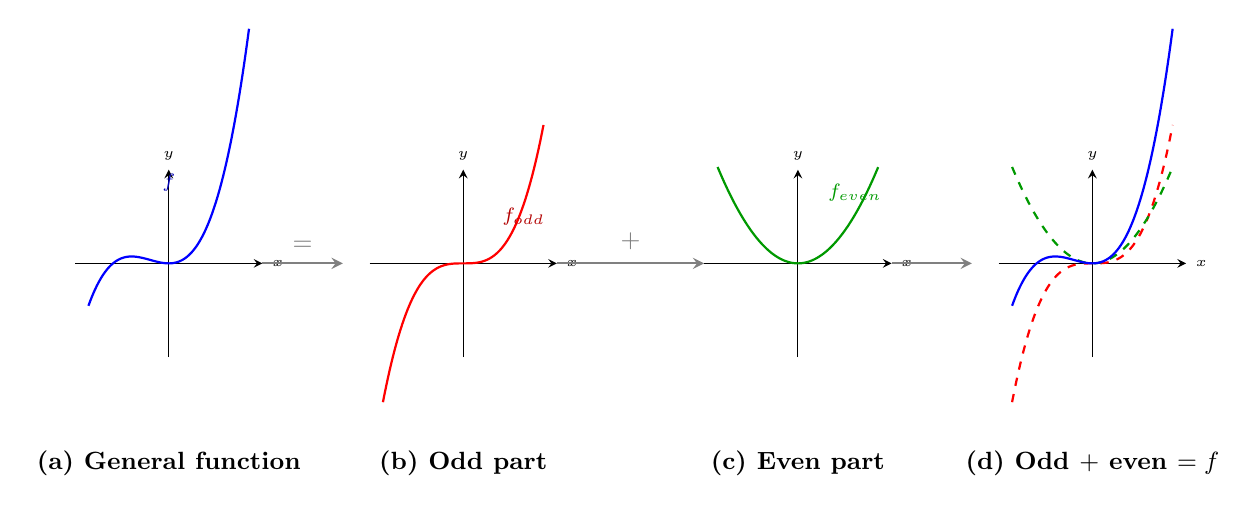
\begin{tikzpicture}[>=stealth, scale=0.85]
    \def\a{1.2}
    \def\b{1.0}
    \foreach \dx in {-4.4, 0, 5.0, 9.4} {
        \begin{scope}[shift={(\dx,0)}]
            \draw[->] (-1.4,0) -- (1.4,0) node[right, font=\tiny] {$x$};
            \draw[->] (0,-1.4) -- (0,1.4) node[above, font=\tiny] {$y$};
        \end{scope}
    }

    \begin{scope}[shift={(-4.4,0)}]
        \draw[thick, blue, domain=-1.2:1.2, samples=100]
            plot (\x, {\a*\x*\x*\x + \b*\x*\x});
        \node[font=\scriptsize, blue!70!black] at (0,1.2) {$f$};
        \node[font=\small\bfseries, below=0.9cm] at (0,-1.6) {(a) General function};
    \end{scope}

    \begin{scope}[shift={(0,0)}]
        \draw[thick, red, domain=-1.2:1.2, samples=100]
            plot (\x, {\a*\x*\x*\x});
        \node[font=\scriptsize, red!70!black] at (0.9,0.7) {$f_{\text{odd}}$};
        \node[font=\small\bfseries, below=0.9cm] at (0,-1.6) {(b) Odd part};
    \end{scope}

    \begin{scope}[shift={(5.0,0)}]
        \draw[thick, green!60!black, domain=-1.2:1.2, samples=100]
            plot (\x, {\b*\x*\x});
        \node[font=\scriptsize, green!60!black] at (0.85,1.05) {$f_{\text{even}}$};
        \node[font=\small\bfseries, below=0.9cm] at (0,-1.6) {(c) Even part};
    \end{scope}

    \begin{scope}[shift={(9.4,0)}]
        \draw[thick, red, domain=-1.2:1.2, samples=100, dashed]
            plot (\x, {\a*\x*\x*\x});
        \draw[thick, green!60!black, domain=-1.2:1.2, samples=100, dashed]
            plot (\x, {\b*\x*\x});
        \draw[thick, blue, domain=-1.2:1.2, samples=100]
            plot (\x, {\a*\x*\x*\x + \b*\x*\x});
        \node[font=\small\bfseries, below=0.9cm] at (0,-1.6) {(d) Odd $+$ even $=f$};
    \end{scope}

    \draw[->, thick, gray] (-3.0,0) -- (-1.8,0);
    \node[font=\small, gray, above] at (-2.4,0.05) {$=$};
    \draw[->, thick, gray] (1.4,0) -- (3.6,0);
    \node[font=\small, gray, above] at (2.5,0.05) {$+$};
    \draw[->, thick, gray] (6.4,0) -- (7.6,0);
\end{tikzpicture}
\caption{Geometric picture of the parity decomposition theorem. Any function $f$ (blue) decomposes uniquely into the sum of an odd part $f_{\text{odd}}$ (red) and an even part $f_{\text{even}}$ (green).}
\label{fig:parity_decomposition}
\end{figure}

\begin{definition}[Directionality---monotonicity]\label{def:monotonicity}
Let $f: I \to \mathbb{R}$, where $I \subseteq \mathbb{R}$ is an interval.
\begin{enumerate}[label=(\roman*)]
    \item If $x_1 < x_2 \implies f(x_1) \le f(x_2)$, then $f$ is said to be \textbf{monotone increasing} on $I$.
    \item If $x_1 < x_2 \implies f(x_1) < f(x_2)$, then $f$ is said to be \textbf{strictly monotone increasing} on $I$.
    \item If $x_1 < x_2 \implies f(x_1) \ge f(x_2)$, then $f$ is said to be \textbf{monotone decreasing} on $I$.
    \item If $x_1 < x_2 \implies f(x_1) > f(x_2)$, then $f$ is said to be \textbf{strictly monotone decreasing} on $I$.
\end{enumerate}
\end{definition}

\begin{proposition}[Existence of the inverse of a strictly monotonic function]\label{prop:strict_monotone_inverse}
If $f: I \to \mathbb{R}$ is strictly monotone on the interval $I$, then $f$ is injective, $f: I \to f(I)$ is bijective, there exists a unique inverse function $f^{-1}: f(I) \to I$, and $f^{-1}$ is also strictly monotone on $f(I)$.
\end{proposition}

\begin{proof}
\textbf{Injectivity}: let $x_1 \neq x_2$. Assume without loss of generality that $x_1 < x_2$. If $f$ is strictly increasing, then $f(x_1) < f(x_2)$, so $f(x_1) \neq f(x_2)$. If $f$ is strictly decreasing, then $f(x_1) > f(x_2)$, so $f(x_1) \neq f(x_2)$. Hence $f$ is injective.

\textbf{Bijectivity}: after restricting the codomain to $f(I)$, the map $f: I \to f(I)$ is surjective (by the definition of $f(I)$) and injective (by the previous step), hence bijective.

\textbf{Existence and uniqueness of the inverse function}: a bijection necessarily has a unique inverse function $f^{-1}: f(I) \to I$.

\textbf{Monotonicity of the inverse function}: suppose $f$ is strictly increasing. Take $y_1, y_2 \in f(I)$ with $y_1 < y_2$, and let $x_1 = f^{-1}(y_1)$, $x_2 = f^{-1}(y_2)$. If $x_1 \ge x_2$, then the strict increase of $f$ gives $y_1 = f(x_1) \ge f(x_2) = y_2$, contradicting $y_1 < y_2$. Hence $x_1 < x_2$, that is, $f^{-1}(y_1) < f^{-1}(y_2)$, so $f^{-1}$ is strictly increasing. The case in which $f$ is strictly decreasing is analogous.
\end{proof}

\begin{definition}[Rotational closure---iterative composition of functions]\label{def:rotation_composition}
Let $f: X \to X$.
\begin{enumerate}[label=(\roman*)]
    \item \textbf{Powers of a function}: $f^0 := \text{id}_X$, $f^{n+1} := f \circ f^n$ ($n \ge 0$).
    \item \textbf{Rotational closure}: if there exists a least positive integer $n \ge 1$ such that $f^n = \text{id}_X$, then $f$ is said to have rotational closure of order $n$.
\end{enumerate}
\end{definition}

\begin{proposition}[Rotational closure implies bijectivity]\label{prop:rotation_closure_bijective}
Let $f: X \to X$. If there exists $n \ge 1$ such that $f^n = \text{id}_X$, then $f$ is a bijection, and $f^{-1} = f^{n-1}$.
\end{proposition}

\begin{proof}
Verify that $f$ is a bijection: $f$ is injective, because if $f(x_1) = f(x_2)$, then $f^n(x_1) = f^{n-1}(f(x_1)) = f^{n-1}(f(x_2)) = f^n(x_2)$, that is, $x_1 = x_2$. $f$ is surjective, because for any $x \in X$, $x = f^n(x) = f(f^{n-1}(x))$, so $x$ is the image of $f^{n-1}(x)$. The inverse of $f$ is $f^{n-1}$: $f \circ f^{n-1} = f^n = \text{id}_X$ and $f^{n-1} \circ f = f^n = \text{id}_X$.
\end{proof}

\begin{remark}[The relationship between function composition and rotation]\label{rem:composition_rotation}
Function composition is itself not a rotation but a \textbf{translation} (left translation $f \mapsto g \circ f$). The reason rotational closure ($f^n = \text{id}$) is called `rotational' is that it corresponds to the notion of a finite-order element: $f$, as an element of the function space $X^X$, has order $n$ and generates the cyclic group $\langle f \rangle \cong C_n$ under the composition operation. This is the concrete realisation, in a function space, of the finite rotational period (definition \ref{def:strict_period} of the `Operations and Periodicity' chapter).
\end{remark}

\begin{definition}[Periodicity---the synergy of symmetry, directionality and rotation]\label{def:periodicity}
A period can be understood as a repetition pattern produced by a function under the joint action of symmetry ($0$-symmetry), directionality ($1$-symmetry) and rotationality ($i$-symmetry). According to which symmetry centre dominates, periodic functions fall into three basic types:
\begin{enumerate}[label=(\roman*)]
    \item \textbf{Translation period ($0$-symmetry dominant)}: let $X \subseteq \mathbb{R}$ satisfy $X + T = X$. If there exists $T > 0$ such that $f(x+T) = f(x)$ for all $x \in X$, then $f$ is said to have translation period $T$.
    \item \textbf{Scaling period ($1$-symmetry dominant)}: let $X \subseteq \mathbb{R}^+$ satisfy $qX = X$. If there exists $q > 0, q \neq 1$ such that $f(qx) = f(x)$ for all $x \in X$, then $f$ is said to have scaling period $q$.
    \item \textbf{Rotational period ($i$-symmetry dominant)}: let $f: \mathbb{C} \to \mathbb{C}$. If there exists $\theta \in (0, 2\pi)$ such that $f(e^{i\theta}z) = f(z)$ for all $z \in \mathbb{C}$, then $f$ is said to have rotational period $\theta$.
\end{enumerate}
\end{definition}

\begin{remark}[Non-triviality of the scaling period]\label{rem:scaling_period_nontrivial}
The scaling period admits no non-trivial continuous solution on $\mathbb{R}$: if $f(qx) = f(x)$ for all $x \in \mathbb{R}$ and $f$ is continuous at $0$, then for any $x \in \mathbb{R}$, $f(x) = \lim_{n\to\infty} f(q^n x) = f(0)$ (when $0 < q < 1$, $q^n x \to 0$; when $q > 1$, use $q^{-n}$). Hence the natural domain of a scaling period is the multiplicative group $\mathbb{R}^+$ (or $\mathbb{C}^\times$), and a non-trivial scaling-periodic function on it is, for example, $f(x) = \sin(2\pi \log_q x)$, which satisfies $f(qx) = \sin(2\pi \log_q(qx)) = \sin(2\pi(\log_q x + 1)) = f(x)$.
\end{remark}

\begin{theorem}[Monotonic intervals of a periodic function within one period]\label{thm:periodic_monotone_intervals}
Let $f: \mathbb{R} \to \mathbb{R}$ be continuous with least positive period $T$. If $f$ is not a constant function, then in any closed interval of length $T$, $f$ has at least one strictly monotone increasing interval and one strictly monotone decreasing interval.
\end{theorem}

\begin{proof}
By the extreme value theorem (theorem \ref{thm:continuous_closed_interval}), $f$ attains its maximum $M$ and its minimum $m$ on $[0,T]$. Since $f$ is not a constant function, $M > m$. Let $f(x_{\max}) = M$ and $f(x_{\min}) = m$, where $x_{\max}, x_{\min} \in [0,T]$.

\textbf{Case 1}: $x_{\min} < x_{\max}$. On the interval $[x_{\min}, x_{\max}]$, the function $f$ rises continuously from $m$ to $M$. If $f$ were nowhere strictly increasing on that interval, then $f$ would be non-increasing there, but $f(x_{\min}) = m < M = f(x_{\max})$, a contradiction. Hence there exists a strictly increasing subinterval. Similarly, on $[x_{\max}, x_{\min}+T]$ the function $f$ falls continuously from $M$ to $m$; if it were nowhere strictly decreasing then it would be non-decreasing, contradicting the endpoint values, so a strictly decreasing subinterval exists.

\textbf{Case 2}: $x_{\max} < x_{\min}$. Symmetrically, there exists a strictly decreasing subinterval in $[x_{\max}, x_{\min}]$ and a strictly increasing subinterval in $[x_{\min}, x_{\max}+T]$.

\textbf{Case 3}: $x_{\min} = x_{\max}$. Then $M = m$, contradicting $M > m$, so this is impossible.

Since $f$ has period $T$, translating the above intervals by integer multiples of $T$ yields the conclusion for any closed interval of length $T$.
\end{proof}

\subsection{\texorpdfstring{Elementary functions}{Elementary functions}}

\begin{definition}[Elementary functions]\label{def:elementary_functions}
The elementary functions comprise: power functions $x^\alpha$, exponential functions $a^x$ ($a>0$), logarithmic functions $\log_a x$, trigonometric functions $\sin x, \cos x, \tan x$ and their inverse functions, together with the functions obtained from these by finitely many arithmetic operations and compositions.
\end{definition}

\begin{remark}[Similarity interpretation of trigonometric functions]\label{rem:trig_similarity}
The trigonometric functions $\sin x$ and $\cos x$ are strictly periodic functions, with period $2\pi$. From the perspective of the `Scalars and Vectors' chapter, $\cos\theta$ and $\sin\theta$ are respectively the cosine similarity and the sine similarity between a unit vector and the reference axis.
\end{remark}

\section{\texorpdfstring{Limits and Continuity}{Limits and Continuity}}

\subsection{\texorpdfstring{Limits of sequences}{Limits of sequences}}

\begin{definition}[Limit of a sequence]\label{def:seq_limit}
Let $\{a_n\}_{n=1}^{\infty}$ be a real sequence and let $L \in \mathbb{R}$. We write $\displaystyle\lim_{n\to\infty} a_n = L$ if
\[\forall \varepsilon > 0,\; \exists N \in \mathbb{N},\; \forall n > N,\; |a_n - L| < \varepsilon.\]
If no such $L$ exists, the sequence is said to diverge.
\end{definition}

\begin{proposition}[Boundedness of a convergent sequence]\label{prop:convergent_bounded}
If the sequence $\{a_n\}$ converges, then $\{a_n\}$ is bounded.
\end{proposition}

\begin{proof}
Let $\lim a_n = A$. Take $\varepsilon = 1$; by the definition of convergence there exists $N \in \mathbb{N}$ such that $|a_n - A| < 1$ whenever $n > N$, whence $|a_n| \le |a_n - A| + |A| < 1 + |A|$.

Let $M = \max\{|a_1|, |a_2|, \dots, |a_N|, 1 + |A|\}$. Then for all $n \in \mathbb{N}$:
- if $n \le N$, then $|a_n| \le M$ (by the definition of $M$);
- if $n > N$, then $|a_n| < 1 + |A| \le M$.

Therefore $\{a_n\}$ is bounded.
\end{proof}

\begin{figure}[htbp]
\centering
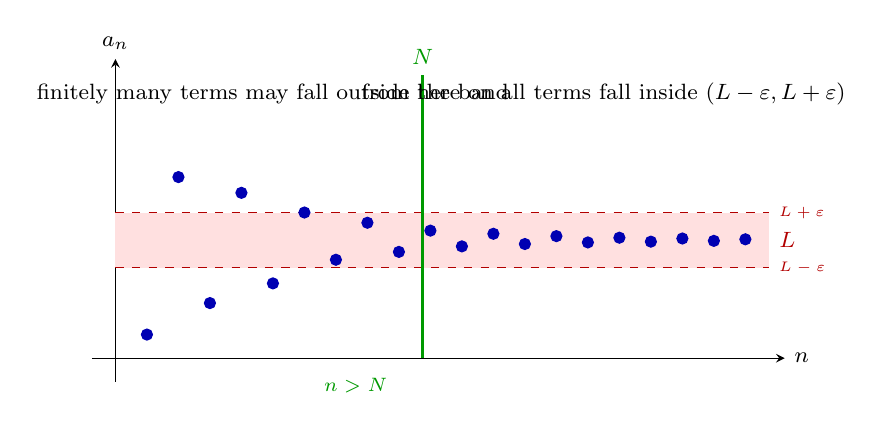
\begin{tikzpicture}[>=stealth, scale=1.0]
    \draw[->] (-0.3,0) -- (8.5,0) node[right, font=\footnotesize] {$n$};
    \draw[->] (0,-0.3) -- (0,3.8) node[above, font=\footnotesize] {$a_n$};

    \draw[thick, red] (0,1.5) -- (8.3,1.5)
        node[right, font=\footnotesize, red!70!black] {$L$};
    \fill[red!12] (0,1.15) rectangle (8.3,1.85);
    \draw[dashed, red!70!black] (0,1.15) -- (8.3,1.15)
        node[right, font=\tiny, red!70!black] {$L-\varepsilon$};
    \draw[dashed, red!70!black] (0,1.85) -- (8.3,1.85)
        node[right, font=\tiny, red!70!black] {$L+\varepsilon$};

    \foreach \n/\y in {0.4/0.3, 0.8/2.3, 1.2/0.7, 1.6/2.1,
                       2.0/0.95, 2.4/1.85, 2.8/1.25, 3.2/1.72,
                       3.6/1.35, 4.0/1.62, 4.4/1.42, 4.8/1.58,
                       5.2/1.45, 5.6/1.55, 6.0/1.47, 6.4/1.53,
                       6.8/1.48, 7.2/1.52, 7.6/1.49, 8.0/1.51} {
        \filldraw[blue!70!black] (\n,\y) circle (2pt);
    }

    \def\NN{3.9}
    \draw[thick, green!60!black] (\NN,0) -- (\NN,3.6)
        node[above, font=\footnotesize, green!60!black] {$N$};
    \node[font=\scriptsize, green!60!black] at (\NN-0.85,-0.35) {$n>N$};

    \node[font=\footnotesize, align=left] at (2.0,3.35)
        {finitely many terms may fall outside the band};
    \node[font=\footnotesize, align=left] at (6.2,3.35)
        {from here on all terms fall inside $(L-\varepsilon,L+\varepsilon)$};
\end{tikzpicture}
\caption{Visualisation of the $\varepsilon$-$N$ definition of the limit of a sequence. The red horizontal line is the limit $L$, and the banded region between the red dashed lines is $(L-\varepsilon,L+\varepsilon)$. All points after $n>N$ fall inside this band.}
\label{fig:seq_limit_epsilon_N}
\end{figure}

\begin{theorem}[Algebraic properties of limits]\label{thm:limit_ops}
If $\lim a_n = A$ and $\lim b_n = B$, then
\begin{enumerate}[label=(\roman*)]
    \item $\lim (a_n \pm b_n) = A \pm B$;
    \item $\lim (a_n b_n) = AB$;
    \item if $B \neq 0$, then $\lim (a_n / b_n) = A/B$.
\end{enumerate}
\end{theorem}

\begin{proof}
\textbf{(i) Addition}: for any $\varepsilon > 0$, since $\lim a_n = A$ and $\lim b_n = B$, there exist $N_1, N_2 \in \mathbb{N}$ such that
\[
n > N_1 \implies |a_n - A| < \frac{\varepsilon}{2}, \qquad n > N_2 \implies |b_n - B| < \frac{\varepsilon}{2}.
\]
Take $N = \max\{N_1, N_2\}$. Then for $n > N$,
\[
|(a_n + b_n) - (A + B)| \le |a_n - A| + |b_n - B| < \frac{\varepsilon}{2} + \frac{\varepsilon}{2} = \varepsilon.
\]
Hence $\lim(a_n + b_n) = A + B$. Subtraction is similar.

\textbf{(ii) Multiplication}: by proposition \ref{prop:convergent_bounded}, $\{a_n\}$ is bounded; let $|a_n| \le M$ for all $n$. For any $\varepsilon > 0$ there exist $N_1, N_2$ such that
\[
n > N_1 \implies |a_n - A| < \frac{\varepsilon}{2(|B| + 1)}, \qquad n > N_2 \implies |b_n - B| < \frac{\varepsilon}{2M}.
\]
Take $N = \max\{N_1, N_2\}$. For $n > N$,
\begin{align*}
|a_n b_n - AB|
&= |a_n(b_n - B) + B(a_n - A)| \\
&\le |a_n||b_n - B| + |B||a_n - A| \\
&< M \cdot \frac{\varepsilon}{2M} + |B| \cdot \frac{\varepsilon}{2(|B|+1)} \\
&< \varepsilon.
\end{align*}
Hence $\lim(a_n b_n) = AB$.

\textbf{(iii) Division}: first we prove that $\lim(1/b_n) = 1/B$ ($B \neq 0$). Since $\lim b_n = B$ and $|B| > 0$, there exists $N_1$ such that $|b_n - B| < |B|/2$ for $n > N_1$, whence $|b_n| > |B|/2$. For any $\varepsilon > 0$ there exists $N_2$ such that $|b_n - B| < \varepsilon |B|^2/2$ for $n > N_2$. Take $N = \max\{N_1, N_2\}$; then for $n > N$,
\[
\left|\frac{1}{b_n} - \frac{1}{B}\right| = \frac{|b_n - B|}{|b_n||B|} < \frac{\varepsilon |B|^2/2}{|B|/2 \cdot |B|} = \varepsilon.
\]
Hence $\lim(1/b_n) = 1/B$. Combining this with (ii): $\lim(a_n/b_n) = \lim(a_n \cdot 1/b_n) = A \cdot 1/B = A/B$.
\end{proof}

\subsection{\texorpdfstring{Limits and continuity of functions}{Limits and continuity of functions}}

\begin{definition}[Limit of a function]\label{def:func_limit}
Let $f$ be defined on some punctured neighbourhood of the point $x_0$. We write $\displaystyle\lim_{x\to x_0} f(x) = L$ if
\[\forall \varepsilon > 0,\; \exists \delta > 0,\; \forall x \in \operatorname{dom}(f),\; 0 < |x - x_0| < \delta \implies |f(x) - L| < \varepsilon.\]
\end{definition}

\begin{definition}[Continuity]\label{def:continuity}
A function $f$ is said to be \textbf{continuous} at the point $x_0$ if $\lim_{x\to x_0} f(x) = f(x_0)$. If $f$ is continuous at every point of an interval $I$, then $f$ is said to be continuous on $I$.
\end{definition}

\begin{figure}[htbp]
\centering
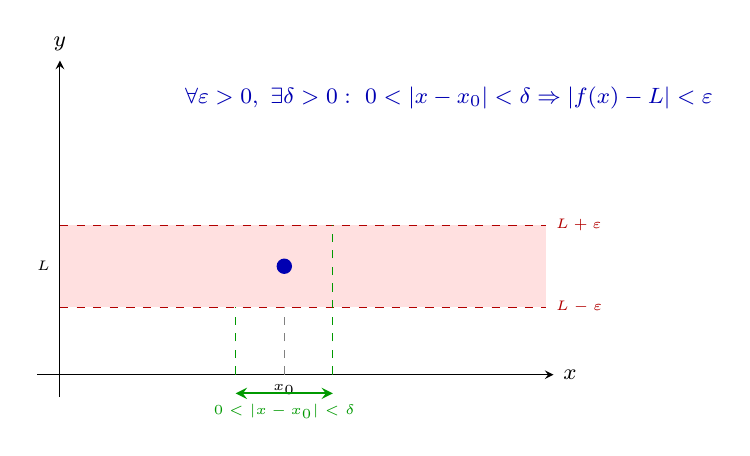
\begin{tikzpicture}[>=stealth, scale=0.95]
    \draw[->] (-0.3,0) -- (6.6,0) node[right, font=\footnotesize] {$x$};
    \draw[->] (0,-0.3) -- (0,4.2) node[above, font=\footnotesize] {$y$};

    \draw[thick, blue!70!black, domain=0.5:5.8, samples=120]
        plot (\x, {1.0 + 0.6*sin(60*\x) + 0.15*\x});

    \def\xz{3.0}
    \pgfmathsetmacro{\yz}{1.0 + 0.6*sin(60*\xz) + 0.15*\xz}

    \draw[dashed, gray] (\xz,0) -- (\xz,\yz);
    \draw[dashed, gray] (0,\yz) -- (\xz,\yz);
    \filldraw[blue!70!black] (\xz,\yz) circle (2.5pt);
    \node[font=\tiny, below] at (\xz,0) {$x_0$};
    \node[font=\tiny, left] at (0,\yz) {$L$};

    \pgfmathsetmacro{\eL}{\yz-0.55}
    \pgfmathsetmacro{\eU}{\yz+0.55}
    \fill[red!12] (0,\eL) rectangle (6.5,\eU);
    \draw[dashed, red!70!black] (0,\eL) -- (6.5,\eL)
        node[right, font=\tiny, red!70!black] {$L-\varepsilon$};
    \draw[dashed, red!70!black] (0,\eU) -- (6.5,\eU)
        node[right, font=\tiny, red!70!black] {$L+\varepsilon$};

    \def\dl{2.35}
    \def\dr{3.65}
    \draw[<->, thick, green!60!black] (\dl,-0.25) -- (\dr,-0.25)
        node[midway, below, font=\tiny, green!60!black]
        {$0<|x-x_0|<\delta$};
    \draw[dashed, green!60!black] (\dl,0) -- (\dl,\eL);
    \draw[dashed, green!60!black] (\dr,0) -- (\dr,\eU);

    \draw[fill=white, thick, blue!70!black] (\xz,\yz) circle (2.5pt);
    \filldraw[blue!70!black] (\xz,\yz) circle (1.5pt);

    \node[font=\footnotesize, blue!70!black, align=center] at (5.2,3.7)
        {$\forall \varepsilon>0,\ \exists \delta>0:\ 0<|x-x_0|<\delta \Rightarrow |f(x)-L|<\varepsilon$};
\end{tikzpicture}
\caption{Visualisation of the $\varepsilon$-$\delta$ definition of the limit of a function. The red horizontal band is $(L-\varepsilon,L+\varepsilon)$, and the green interval is the corresponding $\delta$-neighbourhood. Whenever $x$ falls inside that neighbourhood (other than $x_0$ itself), $f(x)$ must fall inside the $\varepsilon$-band.}
\label{fig:func_limit_epsilon_delta}
\end{figure}

\begin{theorem}[Properties of continuous functions on a closed interval]\label{thm:continuous_closed_interval}
Let $f$ be continuous on the closed interval $[a,b]$. Then:
\begin{enumerate}[label=(\roman*)]
    \item \textbf{Boundedness theorem}: $f$ is bounded on $[a,b]$.
    \item \textbf{Extreme value theorem}: $f$ attains its maximum and minimum on $[a,b]$.
    \item \textbf{Intermediate value theorem}: if $f(a) < c < f(b)$, then there exists $\xi \in (a,b)$ such that $f(\xi) = c$.
    \item \textbf{Uniform continuity theorem}: $f$ is uniformly continuous on $[a,b]$.
\end{enumerate}
\end{theorem}

\begin{proof}
\textbf{(i) Boundedness theorem}: suppose, to the contrary, that $f$ is unbounded on $[a,b]$. Then for each $n \in \mathbb{N}$ there exists $x_n \in [a,b]$ with $|f(x_n)| > n$. By the Bolzano--Weierstrass theorem (a corollary of the completeness of the real numbers in the `Number Systems' chapter), the bounded sequence $\{x_n\}$ has a convergent subsequence $\{x_{n_k}\}$; let its limit be $x_0 \in [a,b]$ (since $[a,b]$ is a closed set). By the continuity of $f$, $\lim_{k\to\infty} f(x_{n_k}) = f(x_0)$. But $|f(x_{n_k})| > n_k \to \infty$, a contradiction. Hence $f$ is bounded.

\textbf{(ii) Extreme value theorem}: by (i), $f$ is bounded on $[a,b]$, so $M := \sup\{f(x) : x \in [a,b]\}$ exists. We must show that there exists $x_0 \in [a,b]$ with $f(x_0) = M$. By the definition of the supremum, for each $n$ there exists $x_n \in [a,b]$ with $M - 1/n < f(x_n) \le M$. By the Bolzano--Weierstrass theorem, $\{x_n\}$ has a convergent subsequence $\{x_{n_k}\} \to x_0 \in [a,b]$. By continuity, $f(x_0) = \lim_{k} f(x_{n_k}) = M$. The case of the minimum is analogous.

\textbf{(iii) Intermediate value theorem}: let $f(a) < c < f(b)$ (the case $f(a) > c > f(b)$ is similar). Construct the set $S = \{x \in [a,b] : f(x) < c\}$. The set $S$ is non-empty ($a \in S$) and has upper bound $b$, so $\xi := \sup S$ exists. We must show that $f(\xi) = c$.

If $f(\xi) < c$, then by the continuity of $f$ at $\xi$ there exists $\delta > 0$ such that every $x \in (\xi-\delta, \xi+\delta) \cap [a,b]$ satisfies $f(x) < c$. In particular, there exists $x > \xi$ with $x \in S$, contradicting the fact that $\xi$ is the supremum of $S$.

If $f(\xi) > c$, then similarly there exists $\delta > 0$ such that every $x \in (\xi-\delta, \xi+\delta) \cap [a,b]$ satisfies $f(x) > c$. This means that $\xi - \delta/2$ is an upper bound for $S$, contradicting the fact that $\xi$ is the least upper bound.

Hence $f(\xi) = c$.

\textbf{(iv) Uniform continuity theorem}: suppose, to the contrary, that $f$ is not uniformly continuous on $[a,b]$. Then there exists $\varepsilon_0 > 0$ such that for each $n$ there exist $x_n, y_n \in [a,b]$ with $|x_n - y_n| < 1/n$ but $|f(x_n) - f(y_n)| \ge \varepsilon_0$. By the Bolzano--Weierstrass theorem, $\{x_n\}$ has a convergent subsequence $\{x_{n_k}\} \to x_0 \in [a,b]$. Since $|x_{n_k} - y_{n_k}| < 1/n_k \to 0$, the sequence $\{y_{n_k}\}$ also converges to $x_0$. By the continuity of $f$, $f(x_{n_k}) \to f(x_0)$ and $f(y_{n_k}) \to f(x_0)$, so $|f(x_{n_k}) - f(y_{n_k})| \to 0$, contradicting $|f(x_{n_k}) - f(y_{n_k})| \ge \varepsilon_0$.
\end{proof}

\begin{figure}[htbp]
\centering
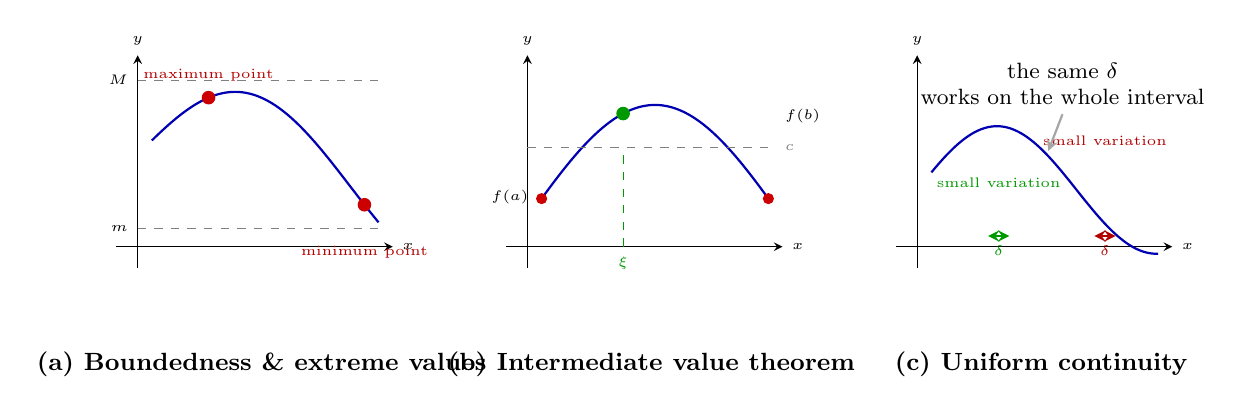
\begin{tikzpicture}[>=stealth, scale=0.9]

    \begin{scope}[shift={(0,0)}]
        \draw[->] (-0.3,0) -- (3.6,0) node[right, font=\tiny] {$x$};
        \draw[->] (0,-0.3) -- (0,2.7) node[above, font=\tiny] {$y$};
        \draw[thick, blue!70!black, domain=0.2:3.4, samples=120]
            plot (\x, {1.3 + 1.1*sin(60*\x) - 0.15*\x});
        \draw[dashed, gray] (0,0.25) -- (3.5,0.25);
        \draw[dashed, gray] (0,2.35) -- (3.5,2.35);
        \node[font=\tiny, left] at (0,2.35) {$M$};
        \node[font=\tiny, left] at (0,0.25) {$m$};
        \filldraw[red!80!black] (1.0,{1.3 + 1.1*sin(60*1.0) - 0.15*1.0}) circle (2.5pt);
        \node[font=\tiny, red!70!black, above] at (1.0,2.2) {maximum point};
        \filldraw[red!80!black] (3.2,{1.3 + 1.1*sin(60*3.2) - 0.15*3.2}) circle (2.5pt);
        \node[font=\tiny, red!70!black, below] at (3.2,0.15) {minimum point};
        \node[font=\small\bfseries, below=0.4cm] at (1.75,-0.9) {(a) Boundedness \& extreme values};
    \end{scope}

    \begin{scope}[shift={(5.5,0)}]
        \draw[->] (-0.3,0) -- (3.6,0) node[right, font=\tiny] {$x$};
        \draw[->] (0,-0.3) -- (0,2.7) node[above, font=\tiny] {$y$};
        \draw[thick, blue!70!black, domain=0.2:3.4, samples=120]
            plot (\x, {0.4 + 1.6*sin(50*\x)});
        \draw[dashed, gray] (0,1.4) -- (3.5,1.4)
            node[right, font=\tiny, gray] {$c$};
        \filldraw[red!80!black] (0.2,{0.4 + 1.6*sin(50*0.2)}) circle (2pt);
        \node[font=\tiny, left] at (0.15,0.7) {$f(a)$};
        \filldraw[red!80!black] (3.4,{0.4 + 1.6*sin(50*3.4)}) circle (2pt);
        \node[font=\tiny, right] at (3.5,1.85) {$f(b)$};
        \filldraw[green!60!black]
            (1.35,{0.4 + 1.6*sin(50*1.35)}) circle (2.5pt);
        \draw[dashed, green!60!black] (1.35,0) -- (1.35,1.4);
        \node[font=\tiny, green!60!black, below] at (1.35,0) {$\xi$};
        \node[font=\small\bfseries, below=0.4cm] at (1.75,-0.9) {(b) Intermediate value theorem};
    \end{scope}

    \begin{scope}[shift={(11,0)}]
        \draw[->] (-0.3,0) -- (3.6,0) node[right, font=\tiny] {$x$};
        \draw[->] (0,-0.3) -- (0,2.7) node[above, font=\tiny] {$y$};
        \draw[thick, blue!70!black, domain=0.2:3.4, samples=120]
            plot (\x, {0.8 + 0.9*sin(80*\x)});
        \draw[<->, thick, green!60!black] (1.0,0.15) -- (1.3,0.15)
            node[midway, below, font=\tiny] {$\delta$};
        \draw[<->, thick, red!70!black] (2.5,0.15) -- (2.8,0.15)
            node[midway, below, font=\tiny] {$\delta$};
        \node[font=\tiny, green!60!black] at (1.15,0.9) {small variation};
        \node[font=\tiny, red!70!black] at (2.65,1.5) {small variation};

        \node[font=\footnotesize, align=center] (cnote) at (2.05, 2.30)
            {the same $\delta$\\works on the whole interval};
        \draw[->, thick, gray!70] (cnote.south) -- (1.85, 1.35);

        \node[font=\small\bfseries, below=0.4cm] at (1.75,-0.9) {(c) Uniform continuity};
    \end{scope}
\end{tikzpicture}
\caption{Three basic properties of continuous functions on a closed interval: (a) boundedness and extreme values; (b) the intermediate value theorem; (c) uniform continuity.}
\label{fig:closed_interval_continuity}
\end{figure}

\section{\texorpdfstring{Derivatives: the directional information of a function}{Derivatives: the directional information of a function}}

\subsection{\texorpdfstring{Definition of the derivative and differentiation rules}{Definition of the derivative and differentiation rules}}

\begin{definition}[Derivative and limit angle]\label{def:derivative}
Let the function $y = f(x)$ be defined on some neighbourhood of the point $x_0$. If the limit
\[f'(x_0) := \lim_{\Delta x \to 0} \frac{f(x_0 + \Delta x) - f(x_0)}{\Delta x}\]
exists and is finite, then $f$ is said to be \textbf{differentiable} at $x_0$, and this limiting value is called the \textbf{derivative} of $f$ at $x_0$. The derivative $f'(x_0)$ is a \textbf{directional quantity}: its sign indicates the direction in which the function changes, and its absolute value indicates the rate of change.

\textbf{Limit angle}: $f'(x_0) = \tan\theta$, and $\theta = \arctan(f'(x_0))$ is called the \textbf{limit angle} of $f$ at $x_0$. The limit angle is the central bridge connecting the vector level (geometric argument) with the function level (calculus direction).
\end{definition}

\begin{figure}[htbp]
\centering
\begin{tikzpicture}[>=stealth, scale=1.0]
    \draw[->] (-3.2,0) -- (10.2,0) node[right, font=\footnotesize] {$x$};
    \draw[->] (0,-1.4) -- (0,5.4) node[above, font=\footnotesize] {$y$};

    \draw[thick, blue!70!black, domain=0.4:5.2, samples=120]
        plot (\x, {0.5 + 0.35*\x + 0.12*(\x-2.8)*(\x-2.8)});

    \def\xz{2.0}
    \pgfmathsetmacro{\yz}{0.5 + 0.35*\xz + 0.12*(\xz-2.8)*(\xz-2.8)}
    \pgfmathsetmacro{\k}{0.35 + 0.24*(\xz-2.8)}
    \pgfmathsetmacro{\ang}{atan(\k)}

    \draw[thick, red] ({\xz-1.4},{\yz-\k*1.4}) -- ({\xz+2.8},{\yz+\k*2.8});

    \def\dx{1.6}
    \pgfmathsetmacro{\xs}{\xz+\dx}
    \pgfmathsetmacro{\ys}{0.5 + 0.35*\xs + 0.12*(\xs-2.8)*(\xs-2.8)}
    \draw[thick, green!60!black, dashed]
        (\xz,\yz) -- (\xs,\ys);

    \draw[dashed, gray] (\xs,\ys) -- (\xs,\yz) -- (\xz,\yz);

    \filldraw[blue!70!black] (\xz,\yz) circle (2.5pt);
    \filldraw[green!60!black] (\xs,\ys) circle (2pt);

    \draw[thick, orange!80!black] ({\xz+1.4},{\yz}) arc (0:\ang:1.4);
    \draw[dashed, orange!50] ({\xz},{\yz}) -- ({\xz+2.4},{\yz});
    \pgfmathsetmacro{\armx}{\xz+1.5*cos(\ang)}
    \pgfmathsetmacro{\army}{\yz+1.5*sin(\ang)}
    \draw[dashed, orange!50] ({\xz},{\yz}) -- (\armx,\army);

    \node[font=\footnotesize] (labx0) at (0.9,-1.0) {$x_0$};
    \draw[->, thick, blue!70!black] (labx0.north) -- ({\xz-0.05},{\yz-0.15});

    \node[font=\footnotesize] (labxs) at (6.014,4.251) {$x_0+\Delta x$};
    \draw[->, thick, green!60!black] (labxs.south west)
        -- ({\xs+0.08},{\ys+0.10});

    \pgfmathsetmacro{\thx}{\xz+1.65*cos(\ang/2)}
    \pgfmathsetmacro{\thy}{\yz+1.65*sin(\ang/2)}
    \node[font=\footnotesize, orange!80!black] (labth) at (\thx,\thy) {$\theta$};

    \node[font=\footnotesize, red!70!black] (labtan) at (-1.7,3.3)
        {tangent slope $=f'(x_0)$};
    \draw[->, thick, red!70!black] (labtan.east) -- (1.5,1.20);

    \pgfmathsetmacro{\midx}{\xz+\dx*0.5}
    \pgfmathsetmacro{\midy}{\yz+(\ys-\yz)*0.5}
    \node[font=\footnotesize, green!60!black] (labsec)
        at (\midx, \midy+1.15) {secant slope $=\dfrac{\Delta y}{\Delta x}$};
    \draw[->, thick, green!60!black] (labsec.south)
        -- (\midx, \midy+0.08);

    \node[font=\footnotesize, orange!80!black] (labang) at (6.57,1.41)
        {limit angle $\theta=\arctan f'(x_0)$};
    \draw[->, thick, orange!80!black] (labang.west)
        -- (\thx+0.15, \thy-0.08);
\end{tikzpicture}
\caption{Geometric interpretation of the derivative and the limit angle. The secant slope tends to the tangent slope $f'(x_0)$ as $\Delta x \to 0$, and $f'(x_0)=\tan\theta$, so $\theta=\arctan f'(x_0)$ is the limit angle of $f$ at $x_0$. The orange auxiliary dashed lines in the figure mark the two sides of $\theta$: the horizontal direction (the positive direction of the $x$-axis) and the tangent direction; $\theta$ is the angle between the two.}
\label{fig:derivative_limit_angle}
\end{figure}

\begin{proposition}[Differentiability implies continuity]\label{prop:diff_implies_cont}
If $f$ is differentiable at $x_0$, then $f$ is continuous at $x_0$.
\end{proposition}

\begin{proof}
\[
\lim_{\Delta x \to 0} [f(x_0+\Delta x) - f(x_0)] = \lim_{\Delta x \to 0} \left( \frac{f(x_0+\Delta x) - f(x_0)}{\Delta x} \cdot \Delta x \right) = f'(x_0) \cdot 0 = 0.
\]
Hence $\lim_{\Delta x \to 0} f(x_0+\Delta x) = f(x_0)$, that is, $f$ is continuous at $x_0$.
\end{proof}

\begin{theorem}[Differentiation rules]\label{thm:derivative_rules}
Let $u(x)$ and $v(x)$ be differentiable at $x$, and let $c$ be a constant.
\begin{enumerate}[label=(\roman*)]
    \item $(c)' = 0$.
    \item $(cu)'(x) = c u'(x)$.
    \item $(u \pm v)'(x) = u'(x) \pm v'(x)$.
    \item $(uv)'(x) = u'(x)v(x) + u(x)v'(x)$.
    \item if $v(x) \neq 0$, then $\left(\frac{u}{v}\right)'(x) = \frac{u'(x)v(x) - u(x)v'(x)}{v(x)^2}$.
\end{enumerate}
\end{theorem}

\begin{proof}
\textbf{(i) Constant}: $\lim_{\Delta x \to 0} \frac{c - c}{\Delta x} = 0$.

\textbf{(ii) Scalar multiple}: $\lim_{\Delta x \to 0} \frac{cu(x+\Delta x) - cu(x)}{\Delta x} = c \lim_{\Delta x \to 0} \frac{u(x+\Delta x) - u(x)}{\Delta x} = cu'(x)$.

\textbf{(iii) Sum and difference}:
\[
\lim_{\Delta x \to 0} \frac{[u(x+\Delta x) \pm v(x+\Delta x)] - [u(x) \pm v(x)]}{\Delta x} = u'(x) \pm v'(x).
\]

\textbf{(iv) Product}:
\[
\frac{(uv)(x+\Delta x) - (uv)(x)}{\Delta x} = u(x+\Delta x)\frac{v(x+\Delta x)-v(x)}{\Delta x} + v(x)\frac{u(x+\Delta x)-u(x)}{\Delta x}.
\]
By the fact that differentiability implies continuity (proposition \ref{prop:diff_implies_cont}), $u(x+\Delta x) \to u(x)$ (as $\Delta x \to 0$). Taking the limit gives $(uv)'(x) = u(x)v'(x) + u'(x)v(x)$.

\textbf{(v) Quotient}: first we prove that $(1/v)' = -v'/v^2$. By the chain rule (theorem \ref{thm:chain_rule}), $(1/v)' = -v'/v^2$ (where $1/v = v^{-1}$, $(v^{-1})' = -v^{-2}v'$). Then, by the product rule, $(u/v)' = (u \cdot v^{-1})' = u'v^{-1} + u(-v^{-2}v') = (u'v - uv')/v^2$.
\end{proof}

\begin{theorem}[Chain rule]\label{thm:chain_rule}
If $u = g(x)$ is differentiable at $x_0$, and $y = f(u)$ is differentiable at $u_0 = g(x_0)$, then
\[(f \circ g)'(x_0) = f'(g(x_0)) \cdot g'(x_0).\]
\end{theorem}

\begin{proof}
Since $f$ is differentiable at $u_0$, there exists a function $\eta(\Delta u)$ satisfying $\lim_{\Delta u \to 0} \eta(\Delta u) = 0$ such that
\[
f(u_0 + \Delta u) - f(u_0) = f'(u_0)\Delta u + \eta(\Delta u)\Delta u.
\]
Let $\Delta u = g(x_0 + \Delta x) - g(x_0)$. Since $g$ is differentiable at $x_0$, $\Delta u = g'(x_0)\Delta x + o(\Delta x)$. Substituting gives
\[
(f \circ g)(x_0 + \Delta x) - (f \circ g)(x_0) = f'(u_0)[g'(x_0)\Delta x + o(\Delta x)] + \eta(\Delta u)\Delta u.
\]
Since $\Delta u \to 0$ (as $\Delta x \to 0$) and $\eta(\Delta u) \to 0$,
\[
\lim_{\Delta x \to 0} \frac{(f \circ g)(x_0 + \Delta x) - (f \circ g)(x_0)}{\Delta x} = f'(u_0)g'(x_0).
\]
\end{proof}

\begin{remark}[Counterexample of continuous but non-differentiable]\label{rem:continuous_not_differentiable}
Continuity does not imply differentiability. Counterexample: $f(x)=|x|$ is continuous at $x=0$. Right derivative:
\[
\lim_{h \to 0^+} \frac{|0+h| - |0|}{h} = \lim_{h \to 0^+} \frac{h}{h} = 1.
\]
Left derivative:
\[
\lim_{h \to 0^-} \frac{|0+h| - |0|}{h} = \lim_{h \to 0^-} \frac{-h}{h} = -1.
\]
The left and right derivatives are unequal, so $f$ is not differentiable at $x=0$.
\end{remark}

\subsection{\texorpdfstring{Mean value theorems of the differential calculus}{Mean value theorems of the differential calculus}}

\begin{theorem}[Fermat's lemma]\label{thm:fermat}
If $f$ is differentiable at $x_0$ and attains a local extremum at $x_0$, then $f'(x_0) = 0$.
\end{theorem}

\begin{proof}
Assume without loss of generality that $f$ attains a local maximum at $x_0$, that is, there exists $\delta > 0$ such that $f(x) \le f(x_0)$ whenever $|x - x_0| < \delta$.

When $\Delta x > 0$ (and $\Delta x < \delta$), we have $f(x_0 + \Delta x) - f(x_0) \le 0$, so
\[
\frac{f(x_0+\Delta x) - f(x_0)}{\Delta x} \le 0.
\]
Taking the limit $\Delta x \to 0^+$ gives the right derivative $f'_+(x_0) \le 0$.

When $\Delta x < 0$ (and $|\Delta x| < \delta$), we have $f(x_0 + \Delta x) - f(x_0) \le 0$, but $\Delta x < 0$, so
\[
\frac{f(x_0+\Delta x) - f(x_0)}{\Delta x} \ge 0.
\]
Taking the limit $\Delta x \to 0^-$ gives the left derivative $f'_-(x_0) \ge 0$.

Since $f$ is differentiable, $f'_+(x_0) = f'_-(x_0) = f'(x_0)$. Therefore $f'(x_0) \le 0$ and $f'(x_0) \ge 0$, so $f'(x_0) = 0$. The case of a local minimum is analogous.
\end{proof}

\begin{theorem}[Rolle's theorem]\label{thm:rolle}
If $f$ is continuous on $[a,b]$, differentiable on $(a,b)$, and $f(a) = f(b)$, then there exists $\xi \in (a,b)$ such that $f'(\xi) = 0$.
\end{theorem}

\begin{proof}
By the extreme value theorem (theorem \ref{thm:continuous_closed_interval}), $f$ attains its maximum $M$ and its minimum $m$ on $[a,b]$.

\textbf{Case 1}: $M = m$. Then $f$ is identically constant, and $f'(x) = 0$ for all $x \in (a,b)$.

\textbf{Case 2}: $M > m$. Since $f(a) = f(b)$, the maximum and the minimum cannot both be attained at the endpoints (if both were attained at the endpoints, then $f(a) = f(b) = M = m$, a contradiction). Hence at least one extremum is attained inside $(a,b)$. Let $f(\xi) = M$ (or $m$) with $\xi \in (a,b)$. By Fermat's lemma (theorem \ref{thm:fermat}), $f'(\xi) = 0$.
\end{proof}

\begin{theorem}[Lagrange's mean value theorem]\label{thm:lagrange}
If $f$ is continuous on $[a,b]$ and differentiable on $(a,b)$, then there exists $\xi \in (a,b)$ such that
\[f(b) - f(a) = f'(\xi)(b-a).\]
\end{theorem}

\begin{proof}
Construct the auxiliary function
\[
\varphi(x) = f(x) - f(a) - \frac{f(b)-f(a)}{b-a}(x-a).
\]
Verify that $\varphi$ satisfies the hypotheses of Rolle's theorem: (i) $\varphi$ is continuous on $[a,b]$ (a continuous function $f$ minus a linear function); (ii) $\varphi$ is differentiable on $(a,b)$; and
\[
\varphi(a) = f(a) - f(a) - 0 = 0, \qquad
\varphi(b) = f(b) - f(a) - \frac{f(b)-f(a)}{b-a}(b-a) = 0.
\]
By Rolle's theorem (theorem \ref{thm:rolle}), there exists $\xi \in (a,b)$ with $\varphi'(\xi) = 0$. Now
\[
\varphi'(x) = f'(x) - \frac{f(b)-f(a)}{b-a}.
\]
Substituting $x = \xi$ gives $f'(\xi) = \frac{f(b)-f(a)}{b-a}$.
\end{proof}

\begin{corollary}[Mean value property of periodic functions]\label{cor:periodic_mean_value}
If $f$ is differentiable on $\mathbb{R}$ and has period $T$, then within one period there exists $\xi \in (x, x+T)$ such that $f'(\xi) = 0$.
\end{corollary}

\begin{proof}
Applying Lagrange's mean value theorem (theorem \ref{thm:lagrange}) to the interval $[x, x+T]$, there exists $\xi \in (x, x+T)$ such that
\[
f(x+T) - f(x) = f'(\xi)T.
\]
By periodicity $f(x+T) = f(x)$, so the left-hand side is zero; hence $f'(\xi)T = 0$, that is, $f'(\xi) = 0$.
\end{proof}

\begin{figure}[htbp]
\centering
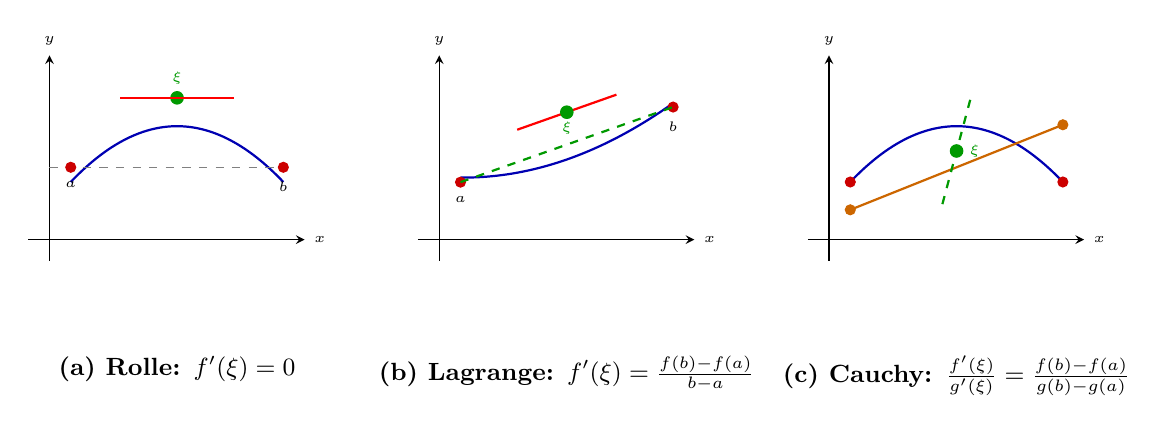
\begin{tikzpicture}[>=stealth, scale=0.9]

    \begin{scope}[shift={(0,0)}]
        \draw[->] (-0.3,0) -- (3.6,0) node[right, font=\tiny] {$x$};
        \draw[->] (0,-0.3) -- (0,2.6) node[above, font=\tiny] {$y$};
        \draw[thick, blue!70!black, domain=0.3:3.3, samples=120]
            plot (\x, {1.6 - 0.35*(\x-1.8)*(\x-1.8)});
        \draw[dashed, gray] (0,1.02) -- (0.3,1.02);
        \draw[dashed, gray] (0,1.02) -- (3.3,1.02);
        \filldraw[red!80!black] (0.3,1.02) circle (2pt);
        \filldraw[red!80!black] (3.3,1.02) circle (2pt);
        \node[font=\tiny, below] at (0.3,0.95) {$a$};
        \node[font=\tiny, below] at (3.3,0.95) {$b$};
        \filldraw[green!60!black] (1.8,2.0) circle (2.5pt);
        \node[font=\tiny, green!60!black, above] at (1.8,2.05) {$\xi$};
        \draw[thick, red] (1.0,2.0) -- (2.6,2.0);
        \node[font=\small\bfseries, below=0.5cm] at (1.8,-0.95)
            {(a) Rolle: $f'(\xi)=0$};
    \end{scope}

    \begin{scope}[shift={(5.5,0)}]
        \draw[->] (-0.3,0) -- (3.6,0) node[right, font=\tiny] {$x$};
        \draw[->] (0,-0.3) -- (0,2.6) node[above, font=\tiny] {$y$};
        \draw[thick, blue!70!black, domain=0.3:3.3, samples=120]
            plot (\x, {0.5 + 0.35*\x + 0.12*(\x-1.8)*(\x-1.8)});
        \filldraw[red!80!black] (0.3,0.81) circle (2pt);
        \filldraw[red!80!black] (3.3,1.87) circle (2pt);
        \node[font=\tiny, below] at (0.3,0.74) {$a$};
        \node[font=\tiny, below] at (3.3,1.8) {$b$};
        \draw[thick, green!60!black, dashed] (0.3,0.81) -- (3.3,1.87);
        \pgfmathsetmacro{\k}{(1.87-0.81)/(3.3-0.3)}
        \draw[thick, red] (1.1,1.55) -- (2.5,1.55+\k*1.4);
        \filldraw[green!60!black] (1.8,1.55+\k*0.7) circle (2.5pt);
        \node[font=\tiny, green!60!black, below] at (1.8,1.55+\k*0.7) {$\xi$};
        \node[font=\small\bfseries, below=0.5cm] at (1.8,-0.95)
            {(b) Lagrange: $f'(\xi)=\frac{f(b)-f(a)}{b-a}$};
    \end{scope}

    \begin{scope}[shift={(11,0)}]
        \draw[->] (-0.3,0) -- (3.6,0) node[right, font=\tiny] {$x$};
        \draw[->] (0,-0.3) -- (0,2.6) node[above, font=\tiny] {$y$};
        \draw[thick, blue!70!black, domain=0.3:3.3, samples=100]
            plot ({\x},{1.6 - 0.35*(\x-1.8)*(\x-1.8)});
        \draw[thick, orange!80!black, domain=0.3:3.3, samples=100]
            plot ({\x},{0.3 + 0.4*\x});
        \filldraw[red!80!black] (0.3,{1.6 - 0.35*(0.3-1.8)*(0.3-1.8)}) circle (2pt);
        \filldraw[red!80!black] (3.3,{1.6 - 0.35*(3.3-1.8)*(3.3-1.8)}) circle (2pt);
        \filldraw[orange!80!black] (0.3,{0.3+0.4*0.3}) circle (2pt);
        \filldraw[orange!80!black] (3.3,{0.3+0.4*3.3}) circle (2pt);
        \draw[thick, green!60!black, dashed]
            (1.6,0.5) -- (2.0,2.0);
        \filldraw[green!60!black] (1.8,1.25) circle (2.5pt);
        \node[font=\tiny, green!60!black, right] at (1.85,1.25) {$\xi$};
        \node[font=\small\bfseries, below=0.5cm] at (1.8,-0.95)
            {(c) Cauchy: $\frac{f'(\xi)}{g'(\xi)}=\frac{f(b)-f(a)}{g(b)-g(a)}$};
    \end{scope}
\end{tikzpicture}
\caption{Geometric pictures of the three mean value theorems: (a) Rolle's theorem; (b) Lagrange's mean value theorem; (c) Cauchy's mean value theorem. The dashed line is the secant, and the solid line is the corresponding parallel tangent.}
\label{fig:mean_value_theorems}
\end{figure}

\subsection{\texorpdfstring{Higher-order derivatives and partial derivatives}{Higher-order derivatives and partial derivatives}}

\begin{proposition}[Directional meaning of higher-order derivatives]\label{prop:higher_derivative_direction}
Let $f$ be $n$ times differentiable at the point $x_0$.
\begin{enumerate}[label=(\roman*)]
    \item \textbf{First-order derivative} $f'(x_0)$: tangent direction, limit angle $\theta^{(1)} = \arctan(f'(x_0))$.
    \item \textbf{Second-order derivative} $f''(x_0)$: concavity direction, limit angle $\theta^{(2)} = \arctan(f''(x_0))$.
    \item \textbf{$n$-th order derivative} $f^{(n)}(x_0)$: a finer bending direction.
\end{enumerate}
\end{proposition}

\begin{proof}
(i) This follows directly from definition \ref{def:derivative}: $f'(x_0) = \tan\theta^{(1)}$, $\theta^{(1)} = \arctan(f'(x_0))$.

(ii) $f''(x_0) = (f')'(x_0)$ is the derivative of the derived function $f'$ at $x_0$. By the definition of the derivative, the sign of $f''(x_0)$ determines the monotonicity of $f'$: $f''(x_0) > 0$ means that $f'$ is increasing near $x_0$ (the function is concave up), whilst $f''(x_0) < 0$ means that $f'$ is decreasing near $x_0$ (the function is concave down). The limit angle $\theta^{(2)} = \arctan(f''(x_0))$ measures the degree of inclination of the `concavity direction'.

(iii) By mathematical induction: $f^{(n)}(x_0) = (f^{(n-1)})'(x_0)$ is the derivative at $x_0$ of the $(n-1)$-th derived function, and it characterises the rate of change of the $(n-1)$-th direction, that is, a `finer bending direction'.
\end{proof}

\begin{definition}[Partial derivative as a single-direction operator]\label{def:partial_derivative}
Let the function $u = f(x, y)$ of two variables be defined on a neighbourhood of the point $(x_0, y_0)$. If the limit
\[\frac{\partial f}{\partial x}(x_0, y_0) := \lim_{\Delta x \to 0} \frac{f(x_0 + \Delta x, y_0) - f(x_0, y_0)}{\Delta x}\]
exists and is finite, then $f$ is said to be \textbf{partially differentiable} with respect to $x$ at $(x_0, y_0)$. The derivative $\frac{\partial f}{\partial y}$ is defined similarly.

The partial derivative $\frac{\partial f}{\partial x}$ is the slope of the tangent at $x_0$ to the curve obtained by intersecting the surface $z = f(x,y)$ with the plane $y = y_0$.
\end{definition}

\begin{definition}[Total differential and directional increment]\label{def:total_differential}
If the total increment of $f(x, y)$ at $(x_0, y_0)$ can be written as
\[\Delta f = A\Delta x + B\Delta y + o\!\left(\sqrt{\Delta x^2 + \Delta y^2}\right),\]
then $f$ is said to be \textbf{differentiable} at $(x_0, y_0)$, and $df = A\,dx + B\,dy$ is the \textbf{total differential}. In this case necessarily $A = \frac{\partial f}{\partial x}$, $B = \frac{\partial f}{\partial y}$.
\end{definition}

\begin{definition}[Gradient as the direction of maximal directional derivative]\label{def:gradient_direction}
The \textbf{gradient} of the function $f(x, y)$ at the point $(x_0, y_0)$ is
\[\nabla f(x_0, y_0) = \left( \frac{\partial f}{\partial x}, \frac{\partial f}{\partial y} \right).\]
The gradient direction is the direction in which the directional derivative attains its maximum, and its modulus equals the maximum rate of change.
\end{definition}

\begin{definition}[Higher-order partial derivatives and mixed partial derivatives]\label{def:higher_partial}
If the partial derivative $\frac{\partial f}{\partial x}$ is itself partially differentiable, then
\[\frac{\partial^2 f}{\partial x^2} = \frac{\partial}{\partial x}\left(\frac{\partial f}{\partial x}\right),\quad
\frac{\partial^2 f}{\partial y \partial x} = \frac{\partial}{\partial y}\left(\frac{\partial f}{\partial x}\right)\]
are called second-order partial derivatives.
\end{definition}

\begin{proposition}[Relationship between differentiability and partial derivatives]\label{prop:diff_partial}
If $f$ is differentiable at $(x_0, y_0)$, then both first-order partial derivatives exist. Conversely, the existence of the partial derivatives does not guarantee differentiability.
\end{proposition}

\begin{proof}
\textbf{Forward direction}: let $f$ be differentiable at $(x_0, y_0)$. Then
\[
\Delta f = A\Delta x + B\Delta y + o\!\left(\sqrt{\Delta x^2 + \Delta y^2}\right).
\]
Taking $\Delta y = 0$ gives
\[
f(x_0 + \Delta x, y_0) - f(x_0, y_0) = A\Delta x + o(|\Delta x|).
\]
Dividing by $\Delta x$ and taking the limit:
\[
\frac{\partial f}{\partial x}(x_0, y_0) = \lim_{\Delta x \to 0} \frac{f(x_0+\Delta x, y_0) - f(x_0, y_0)}{\Delta x} = A.
\]
Similarly $\frac{\partial f}{\partial y}(x_0, y_0) = B$.

\textbf{Converse direction (counterexample)}: see note \ref{rem:partial_not_differentiable}.
\end{proof}

\begin{lemma}[Existence of the directional derivative]\label{lem:directional_derivative}
If $f$ is differentiable at $(x_0, y_0)$, then for any unit direction vector $\boldsymbol{l} = (\cos\alpha, \cos\beta)$, the directional derivative
\[\frac{\partial f}{\partial \boldsymbol{l}} = \nabla f \cdot \boldsymbol{l} = f_x \cos\alpha + f_y \cos\beta\]
exists.
\end{lemma}

\begin{proof}
By the definition of the total differential (definition \ref{def:total_differential}),
\[
f(x_0 + t\cos\alpha, y_0 + t\cos\beta) - f(x_0, y_0) = f_x(x_0,y_0)\,t\cos\alpha + f_y(x_0,y_0)\,t\cos\beta + o(t).
\]
Dividing by $t$ and letting $t \to 0$:
\[
\frac{\partial f}{\partial \boldsymbol{l}}(x_0, y_0) = \lim_{t \to 0} \frac{f(x_0 + t\cos\alpha, y_0 + t\cos\beta) - f(x_0, y_0)}{t} = f_x \cos\alpha + f_y \cos\beta = \nabla f \cdot \boldsymbol{l}.
\]
\end{proof}

\begin{theorem}[Multivariable chain rule]\label{thm:multivariable_chain_rule}
Let $u = f(x, y)$ be differentiable and let $x = x(t), y = y(t)$ be differentiable; then
\[\frac{du}{dt} = \frac{\partial f}{\partial x}\frac{dx}{dt} + \frac{\partial f}{\partial y}\frac{dy}{dt}.\]
\end{theorem}

\begin{proof}
Since $f$ is differentiable,
\[
\Delta f = \frac{\partial f}{\partial x}\Delta x + \frac{\partial f}{\partial y}\Delta y + o\!\left(\sqrt{\Delta x^2 + \Delta y^2}\right).
\]
Since $x(t), y(t)$ are differentiable,
\[
\Delta x = x'(t)\Delta t + o(\Delta t), \qquad \Delta y = y'(t)\Delta t + o(\Delta t).
\]
Substituting gives
\[
\Delta f = \left( \frac{\partial f}{\partial x}x'(t) + \frac{\partial f}{\partial y}y'(t) \right)\Delta t + o(\Delta t).
\]
Dividing by $\Delta t$ and taking the limit gives the result.
\end{proof}

\begin{theorem}[Equality of mixed partial derivatives (Clairaut's theorem)]\label{thm:clairaut}
If $f_{xy}$ and $f_{yx}$ are continuous on a neighbourhood of the point $(x_0, y_0)$, then
\[\frac{\partial^2 f}{\partial x \partial y}(x_0, y_0) = \frac{\partial^2 f}{\partial y \partial x}(x_0, y_0).\]
\end{theorem}

\begin{proof}
Consider the second-order difference
\[
\Delta(h,k) = f(x_0+h, y_0+k) - f(x_0+h, y_0) - f(x_0, y_0+k) + f(x_0, y_0).
\]
Define $\varphi(x) = f(x, y_0+k) - f(x, y_0)$. Then
\[
\Delta(h,k) = \varphi(x_0+h) - \varphi(x_0).
\]
By Lagrange's mean value theorem, there exists $\xi$ between $x_0$ and $x_0+h$ such that
\[
\Delta(h,k) = h\varphi'(\xi) = h[f_x(\xi, y_0+k) - f_x(\xi, y_0)].
\]
Applying the mean value theorem again in $y$, there exists $\eta$ between $y_0$ and $y_0+k$ such that
\[
\Delta(h,k) = hk\, f_{xy}(\xi, \eta).
\]
Similarly, define $\psi(y) = f(x_0+h, y) - f(x_0, y)$; then
\[
\Delta(h,k) = \psi(y_0+k) - \psi(y_0) = k\psi'(\eta') = k[f_y(x_0+h, \eta') - f_y(x_0, \eta')] = hk\, f_{yx}(\xi', \eta').
\]
Hence
\[
f_{xy}(\xi, \eta) = f_{yx}(\xi', \eta').
\]
Letting $(h,k) \to (0,0)$, we have $(\xi,\eta) \to (x_0,y_0)$ and $(\xi',\eta') \to (x_0,y_0)$. By the continuity of $f_{xy}$ and $f_{yx}$,
\[
f_{xy}(x_0,y_0) = f_{yx}(x_0,y_0).
\]
\end{proof}

\begin{remark}[Counterexample of partial differentiability without differentiability]\label{rem:partial_not_differentiable}
$f(x,y) = \frac{xy}{x^2+y^2}$ (with $f(0,0)=0$). At $(0,0)$:
\[
\frac{\partial f}{\partial x}(0,0) = \lim_{\Delta x \to 0} \frac{f(\Delta x, 0) - f(0,0)}{\Delta x} = \lim_{\Delta x \to 0} \frac{0 - 0}{\Delta x} = 0,
\]
and similarly $\frac{\partial f}{\partial y}(0,0) = 0$. But the limit along the line $y = kx$ is
\[
\lim_{x \to 0} f(x, kx) = \lim_{x \to 0} \frac{kx^2}{x^2 + k^2x^2} = \frac{k}{1+k^2},
\]
which varies with $k$; hence $f$ is discontinuous at $(0,0)$, and a fortiori not differentiable.
\end{remark}

\section{\texorpdfstring{Differentials: the linear approximation of a function}{Differentials: the linear approximation of a function}}

\begin{definition}[Differential as the linear principal part of the directional increment]\label{def:differential}
Let $y = f(x)$ be differentiable at $x_0$. If the increment
\[\Delta y = f(x_0 + \Delta x) - f(x_0) = f'(x_0)\,\Delta x + o(\Delta x) \quad (\Delta x \to 0),\]
then $dy := f'(x_0)\,dx$ is called the \textbf{differential} of $f$ at $x_0$.
\end{definition}

\begin{lemma}[Consistency of differential and derivative operations]\label{lem:differential_rules}
Let $u(x), v(x)$ be differentiable at $x$ and let $c$ be a constant; then
\begin{enumerate}[label=(\roman*)]
    \item $d(c) = 0$;
    \item $d(cu) = c\,du$;
    \item $d(u \pm v) = du \pm dv$;
    \item $d(uv) = v\,du + u\,dv$;
    \item $d\!\left(\frac{u}{v}\right) = \frac{v\,du - u\,dv}{v^2}\;(v \neq 0)$.
\end{enumerate}
\end{lemma}

\begin{proof}
(i) $d(c) = c'\,dx = 0 \cdot dx = 0$.

(ii) $d(cu) = (cu)'\,dx = cu'\,dx = c\,du$.

(iii) $d(u \pm v) = (u \pm v)'\,dx = (u' \pm v')\,dx = du \pm dv$.

(iv) $d(uv) = (uv)'\,dx = (u'v + uv')\,dx = v(u'\,dx) + u(v'\,dx) = v\,du + u\,dv$.

(v) $d(u/v) = (u/v)'\,dx = \frac{u'v - uv'}{v^2}\,dx = \frac{v(u'\,dx) - u(v'\,dx)}{v^2} = \frac{v\,du - u\,dv}{v^2}$.

Each of the steps above follows directly from the differentiation rules (theorem \ref{thm:derivative_rules}).
\end{proof}

\begin{theorem}[Invariance of the first differential form]\label{thm:invariance_differential}
Let $y = f(u)$ and $u = g(x)$ be differentiable; then $dy = f'(u)\,du = f'(g(x))\,g'(x)\,dx$.
\end{theorem}

\begin{proof}
By the chain rule (theorem \ref{thm:chain_rule}), $(f \circ g)'(x) = f'(g(x))\,g'(x)$. Hence
\[
dy = (f \circ g)'(x)\,dx = f'(g(x))\,g'(x)\,dx.
\]
On the other hand, $du = g'(x)\,dx$, so $f'(u)\,du = f'(g(x))\,g'(x)\,dx$. The two are equal.
\end{proof}

\begin{corollary}[Linear approximation property of differentials]\label{cor:linear_approximation}
If $f$ is differentiable at $x_0$, then for $|x - x_0|$ sufficiently small,
\[f(x) \approx f(x_0) + f'(x_0)(x - x_0).\]
\end{corollary}

\begin{proof}
By the definition of the differential (definition \ref{def:differential}),
\[
f(x) - f(x_0) = f'(x_0)(x - x_0) + o(|x - x_0|).
\]
As $|x - x_0| \to 0$, the quantity $o(|x-x_0|)$ tends to zero faster than $|x-x_0|$; hence
\[
f(x) = f(x_0) + f'(x_0)(x - x_0) + o(|x - x_0|) \approx f(x_0) + f'(x_0)(x - x_0).
\]
\end{proof}

\section{\texorpdfstring{Integration: the tendency information of a function}{Integration: the tendency information of a function}}

\subsection{\texorpdfstring{Integrals in one variable}{Integrals in one variable}}

\begin{definition}[Indefinite integral as the inverse operation of direction]\label{def:indefinite_integral}
Let $f$ be continuous on an interval $I$. If there exists a differentiable function $F$ such that $F'(x) = f(x)$ for all $x \in I$, then $F$ is called an \textbf{antiderivative} of $f$. The set of all antiderivatives of $f$ is called the \textbf{indefinite integral} and is written
\[\int f(x)\,dx = F(x) + C.\]
\end{definition}

\begin{definition}[Riemann integral]\label{def:riemann_integral}
Let $f$ be bounded on $[a,b]$. For a partition $\mathcal{P}: a = x_0 < x_1 < \cdots < x_n = b$, choose arbitrary points $\xi_i \in [x_{i-1}, x_i]$ and form the Riemann sum
\[S(f, \mathcal{P}, \{\xi_i\}) = \sum_{i=1}^{n} f(\xi_i)\,\Delta x_i.\]
If the limit as $\|\mathcal{P}\| \to 0$ exists and is independent of the partition and of the manner in which the points are chosen, then $f$ is said to be \textbf{Riemann integrable} on $[a,b]$, and the limiting value is called the \textbf{definite integral}, written $\int_a^b f(x)\,dx$.
\end{definition}

\begin{theorem}[Fundamental theorem of calculus---the duality of direction and tendency]\label{thm:ftc}
Let $f$ be continuous on $[a,b]$.
\begin{enumerate}[label=(\roman*)]
    \item The integral with variable upper limit $\Phi(x) = \int_a^x f(t)\,dt$ is differentiable on $[a,b]$, and $\Phi'(x) = f(x)$.
    \item If $F$ is any antiderivative of $f$, then $\int_a^b f(x)\,dx = F(b) - F(a)$.
\end{enumerate}
\end{theorem}

\begin{proof}
\textbf{(i)} For $\Delta x > 0$ (the case $\Delta x < 0$ is similar),
\[
\frac{\Phi(x+\Delta x) - \Phi(x)}{\Delta x} = \frac{1}{\Delta x}\int_x^{x+\Delta x} f(t)\,dt.
\]
By the extreme value theorem for continuous functions on a closed interval, $f$ attains its minimum $m(\Delta x)$ and its maximum $M(\Delta x)$ on $[x, x+\Delta x]$, so
\[
m(\Delta x) \le \frac{1}{\Delta x}\int_x^{x+\Delta x} f(t)\,dt \le M(\Delta x).
\]
As $\Delta x \to 0^+$, the continuity of $f$ gives $m(\Delta x) \to f(x)$ and $M(\Delta x) \to f(x)$. By the sandwich theorem,
\[
\lim_{\Delta x \to 0^+} \frac{\Phi(x+\Delta x) - \Phi(x)}{\Delta x} = f(x).
\]
Similarly the left derivative is also $f(x)$. Hence $\Phi'(x) = f(x)$.

\textbf{(ii)} Let $G(x) = \Phi(x) - F(x)$. By (i), $G'(x) = \Phi'(x) - F'(x) = f(x) - f(x) = 0$. By the corollary to Lagrange's mean value theorem (a function whose derivative is zero is constant), $G$ is constant on $[a,b]$. Therefore
\[
\Phi(b) - F(b) = G(b) = G(a) = \Phi(a) - F(a) = -F(a).
\]
Hence $\Phi(b) = F(b) - F(a)$, that is, $\int_a^b f(x)\,dx = F(b) - F(a)$.
\end{proof}

\begin{corollary}[The mutual invertibility of differentiation and integration]\label{cor:diff_int_inverse}
If $f$ is continuous, then
\[\frac{d}{dx}\left( \int_a^x f(t)\,dt \right) = f(x),\qquad
\int_a^b F'(x)\,dx = F(b) - F(a).\]
\end{corollary}

\begin{proof}
The first formula is given directly by theorem \ref{thm:ftc} (i). The second is given directly by theorem \ref{thm:ftc} (ii) applied to $F' = f$.
\end{proof}

\begin{figure}[htbp]
\centering
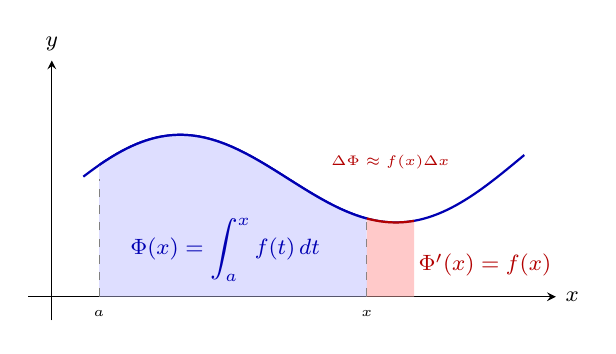
\begin{tikzpicture}[>=stealth, scale=1.0]
    \draw[->] (-0.3,0) -- (6.4,0) node[right, font=\footnotesize] {$x$};
    \draw[->] (0,-0.3) -- (0,3.0) node[above, font=\footnotesize] {$y$};

    \draw[thick, blue!70!black, domain=0.4:6.0, samples=120]
        plot (\x, {1.2 + 0.7*sin(60*\x) + 0.10*\x});

    \def\a{0.6}
    \def\xz{4.0}
    \fill[blue!20, opacity=0.65]
        ({\a},0) -- plot[domain=\a:\xz, samples=100]
        (\x, {1.2 + 0.7*sin(60*\x) + 0.10*\x}) -- (\xz,0) -- cycle;
    \draw[thick, blue!70!black, domain=\a:\xz, samples=100]
        plot (\x, {1.2 + 0.7*sin(60*\x) + 0.10*\x});
    \draw[dashed, gray] (\a,0) -- (\a,1.5);
    \draw[dashed, gray] (\xz,0) -- (\xz,{1.2 + 0.7*sin(60*\xz) + 0.10*\xz});
    \node[font=\tiny, below] at (\a,-0.05) {$a$};
    \node[font=\tiny, below] at (\xz,-0.05) {$x$};

    \node[font=\footnotesize, blue!70!black] at (2.2,0.6)
        {$\Phi(x)=\displaystyle\int_a^x f(t)\,dt$};

    \def\dx{0.6}
    \pgfmathsetmacro{\xu}{\xz+\dx}
    \pgfmathsetmacro{\hu}{1.2 + 0.7*sin(60*\xu) + 0.10*\xu}
    \fill[red!30, opacity=0.7]
        (\xz,0) -- plot[domain=\xz:\xu, samples=40]
        (\x, {1.2 + 0.7*sin(60*\x) + 0.10*\x}) -- (\xu,0) -- cycle;
    \draw[thick, red!70!black, domain=\xz:\xu, samples=40]
        plot (\x, {1.2 + 0.7*sin(60*\x) + 0.10*\x});
    \node[font=\tiny, red!70!black, above] at (\xz+0.3,1.5)
        {$\Delta\Phi\approx f(x)\Delta x$};

    \node[font=\footnotesize, red!70!black] at (5.5,0.4)
        {$\Phi'(x)=f(x)$};
\end{tikzpicture}
\caption{Geometric picture of the fundamental theorem of calculus. The integral with variable upper limit $\Phi(x)$ is the area under the curve, and its increment satisfies $\Delta\Phi \approx f(x)\Delta x$---this is the geometric meaning of $\Phi'(x)=f(x)$.}
\label{fig:ftc_area}
\end{figure}

\begin{property}[Basic properties of the definite integral]\label{prop:integral_properties}
Let $f, g$ be integrable on $[a,b]$ and let $c \in [a,b]$. Then:
\begin{enumerate}[label=(\roman*)]
    \item \textbf{Linearity}: $\int_a^b (f + cg)\,dx = \int_a^b f\,dx + c\int_a^b g\,dx$;
    \item \textbf{Additivity over intervals}: $\int_a^b f\,dx = \int_a^c f\,dx + \int_c^b f\,dx$;
    \item \textbf{Order preservation}: if $f \le g$, then $\int_a^b f\,dx \le \int_a^b g\,dx$;
    \item \textbf{Absolute value estimate}: $\left|\int_a^b f\,dx\right| \le \int_a^b |f|\,dx$.
\end{enumerate}
\end{property}

\begin{proof}
(i) By the linearity of Riemann sums and the linearity of limits:
\[
\int_a^b (f+cg) = \lim \sum (f(\xi_i) + cg(\xi_i))\Delta x_i = \lim \sum f(\xi_i)\Delta x_i + c\lim \sum g(\xi_i)\Delta x_i.
\]

(ii) Any partition of $[a,b]$ can be refined by inserting $c$ as a division point; the identity $\int_a^b f = \int_a^c f + \int_c^b f$ follows directly from the additivity of Riemann sums.

(iii) If $f \le g$, then for any Riemann sum, $\sum f(\xi_i)\Delta x_i \le \sum g(\xi_i)\Delta x_i$. Taking the limit gives the result.

(iv) From $-|f| \le f \le |f|$ and (iii),
\[
-\int_a^b |f|\,dx \le \int_a^b f\,dx \le \int_a^b |f|\,dx,
\]
that is, $\left|\int_a^b f\,dx\right| \le \int_a^b |f|\,dx$.
\end{proof}

\subsection{\texorpdfstring{Integrals in several variables}{Integrals in several variables}}

\begin{definition}[Double integral]\label{def:double_integral}
Let $f(x,y)$ be bounded on a bounded closed region $D \subset \mathbb{R}^2$. Divide $D$ into $n$ subregions $\Delta D_i$, choose arbitrary points $(\xi_i, \eta_i) \in \Delta D_i$, and form the Riemann sum
\[S = \sum_{i=1}^n f(\xi_i, \eta_i)\,\Delta A_i.\]
If the limit exists, then $f$ is said to be \textbf{integrable} on $D$, and the limit is called the \textbf{double integral}:
\[\iint_D f(x,y)\,dA = \lim_{\|\mathcal{P}\| \to 0} \sum_{i=1}^n f(\xi_i, \eta_i)\,\Delta A_i.\]
\end{definition}

\begin{definition}[Triple integral]\label{def:triple_integral}
Let $\Omega \subseteq \mathbb{R}^3$ be a region in space. The \textbf{triple integral} of $f$ over $\Omega$ is defined as
\[\iiint_\Omega f(x, y, z)\,dV.\]
The triple integral is the accumulation of tendency in three dimensions.
\end{definition}

\begin{lemma}[Integral mean value theorem]\label{lem:integral_mean_value}
If $f$ is continuous on a bounded closed region $D$, then there exists $(\xi, \eta) \in D$ such that
\[\iint_D f(x,y)\,dA = f(\xi, \eta) \cdot \mathrm{Area}(D).\]
\end{lemma}

\begin{proof}
By the extreme value theorem, $f$ attains its minimum $m$ and its maximum $M$ on $D$. Then
\[
m \cdot \mathrm{Area}(D) \le \iint_D f(x,y)\,dA \le M \cdot \mathrm{Area}(D).
\]
Hence
\[
m \le \frac{\iint_D f(x,y)\,dA}{\mathrm{Area}(D)} \le M.
\]
By the intermediate value theorem ($D$ is a connected set and $f(D)$ is an interval), there exists $(\xi, \eta) \in D$ such that
\[
f(\xi, \eta) = \frac{\iint_D f(x,y)\,dA}{\mathrm{Area}(D)}.
\]
\end{proof}

\begin{theorem}[Fubini's theorem---iterated integrals and the decomposition of direction]\label{thm:fubini}
If $f(x,y)$ is continuous on the rectangular region $D = [a,b] \times [c,d]$, then
\[\iint_D f(x,y)\,dA = \int_a^b \left( \int_c^d f(x,y)\,dy \right) dx = \int_c^d \left( \int_a^b f(x,y)\,dx \right) dy.\]
\end{theorem}

\begin{proof}
We prove the first equality (the second is analogous).

\textbf{Step 1}: define $F(x) = \int_c^d f(x,y)\,dy$. We must show that $F$ is continuous on $[a,b]$.

For any $x_1, x_2 \in [a,b]$,
\[
|F(x_1) - F(x_2)| \le \int_c^d |f(x_1,y) - f(x_2,y)|\,dy.
\]
By the uniform continuity of $f$ on a bounded closed rectangle (the multivariable version of theorem \ref{thm:continuous_closed_interval}), for any $\varepsilon > 0$ there exists $\delta > 0$ such that $|x_1 - x_2| < \delta$ implies $|f(x_1,y) - f(x_2,y)| < \varepsilon/(d-c)$ for all $y \in [c,d]$. Hence $|F(x_1) - F(x_2)| < \varepsilon$, so $F$ is uniformly continuous.

\textbf{Step 2}: prove that $\iint_D f = \int_a^b F(x)\,dx$.

Divide $[a,b]$ into $m$ equal parts and $[c,d]$ into $n$ equal parts, obtaining a grid partition $\mathcal{P}$. Put $m_{ij} = \inf\{f(x,y) : x \in [x_{i-1}, x_i], y \in [y_{j-1}, y_j]\}$ and $M_{ij} = \sup\{f(x,y) : x \in [x_{i-1}, x_i], y \in [y_{j-1}, y_j]\}$.

The lower and upper sums are respectively
\[
L(\mathcal{P}) = \sum_{i,j} m_{ij}\Delta x_i \Delta y_j, \qquad U(\mathcal{P}) = \sum_{i,j} M_{ij}\Delta x_i \Delta y_j.
\]
For each fixed $x \in [x_{i-1}, x_i]$,
\[
\sum_j m_{ij}\Delta y_j \le \int_c^d f(x,y)\,dy = F(x) \le \sum_j M_{ij}\Delta y_j.
\]
Integrating with respect to $x$ over $[x_{i-1}, x_i]$:
\[
\sum_j m_{ij}\Delta y_j \cdot \Delta x_i \le \int_{x_{i-1}}^{x_i} F(x)\,dx \le \sum_j M_{ij}\Delta y_j \cdot \Delta x_i.
\]
Summing over $i$:
\[
L(\mathcal{P}) \le \int_a^b F(x)\,dx \le U(\mathcal{P}).
\]
Since $f$ is integrable, $\lim_{\|\mathcal{P}\|\to 0} L(\mathcal{P}) = \lim_{\|\mathcal{P}\|\to 0} U(\mathcal{P}) = \iint_D f$. By the sandwich theorem,
\[
\int_a^b F(x)\,dx = \iint_D f(x,y)\,dA.
\]
\end{proof}

\begin{proposition}[Change of variables for multiple integrals]\label{prop:change_of_variables}
Let $\mathbf{T}: D^* \to D$ be a bijective transformation, $(u, v) \mapsto (x(u,v), y(u,v))$. Then
\[\iint_D f(x, y)\,dA = \iint_{D^*} f(x(u,v), y(u,v)) \left|\frac{\partial(x, y)}{\partial(u, v)}\right|\,du\,dv,\]
where $\frac{\partial(x, y)}{\partial(u, v)}$ is the Jacobi determinant, which measures the local area scaling factor of the transformation.
\end{proposition}

\begin{proof}
Divide $D^*$ into small rectangles $[u_i, u_i+\Delta u] \times [v_j, v_j+\Delta v]$. Under $\mathbf{T}$, such a small rectangle is mapped approximately to a parallelogram in $D$, whose two sides are
\[
\mathbf{T}(u_i+\Delta u, v_j) - \mathbf{T}(u_i, v_j) \approx \frac{\partial \mathbf{T}}{\partial u}\Delta u, \qquad
\mathbf{T}(u_i, v_j+\Delta v) - \mathbf{T}(u_i, v_j) \approx \frac{\partial \mathbf{T}}{\partial v}\Delta v.
\]
The area of this parallelogram is
\[
\left\|\frac{\partial \mathbf{T}}{\partial u} \times \frac{\partial \mathbf{T}}{\partial v}\right\| \Delta u \Delta v = \left|\frac{\partial(x,y)}{\partial(u,v)}\right| \Delta u \Delta v.
\]
Hence the Riemann sums satisfy
\[
\sum f(x_i, y_j)\Delta A_{ij} \approx \sum f(\mathbf{T}(u_i, v_j)) \left|\frac{\partial(x,y)}{\partial(u,v)}\right| \Delta u \Delta v.
\]
Taking the limit gives the change-of-variables formula.
\end{proof}

\begin{example}[Triple integral in spherical coordinates]\label{ex:spherical_coordinates}
In spherical coordinates $(r, \theta, \phi)$, the volume element is $dV = r^2 \sin\theta \, dr\, d\theta\, d\phi$. The factor $r^2$ is the manifestation of the inverse-square law in the integration measure.
\end{example}

\section{\texorpdfstring{The limit angle and differential similarity}{The limit angle and differential similarity}}

\begin{figure}[htbp]
\centering
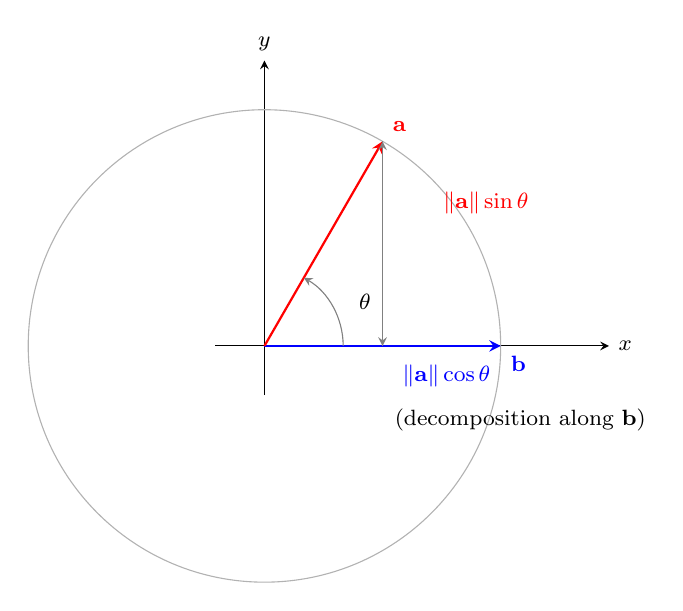
\begin{tikzpicture}[scale=1.25,>=stealth]
    \draw[->] (-0.5,0) -- (3.5,0) node[right] {\footnotesize $x$};
    \draw[->] (0,-0.5) -- (0,2.9) node[above] {\footnotesize $y$};
    \draw[gray!60] (0,0) circle (2.4);
    \draw[->,thick,blue] (0,0) -- (2.4,0) node[below right] {\footnotesize $\mathbf b$};
    \draw[->,thick,red] (0,0) -- (60:2.4) node[above right] {\footnotesize $\mathbf a$};
    \draw[->,gray] (0.8,0) arc (0:60:0.8);
    \node[font=\footnotesize] at (1.02,0.45) {$\theta$};
    \draw[dashed,gray] (60:2.4) -- (1.2,0);
    \draw[<->,gray] (1.2,0) -- (1.2,2.078);
    \node[font=\footnotesize,blue] at (1.85,-0.30) {$\|\mathbf a\|\cos\theta$};
    \node[font=\footnotesize,red] at (2.25,1.45) {$\|\mathbf a\|\sin\theta$};
    \node[font=\footnotesize] at (2.6,-0.75) {(decomposition along $\mathbf b$)};
\end{tikzpicture}
\caption{The limit angle and decomposition along a direction. Decompose $\mathbf a$ orthogonally along the direction of $\mathbf b$: the component along the direction, $\|\mathbf a\|\cos\theta$, measures the \textbf{degree of agreement of direction} (the cosine family), whilst the perpendicular component $\|\mathbf a\|\sin\theta$ measures the \textbf{degree of deviation of direction} (the sine family). Their normalised versions $\cos\theta$ and $\sin\theta$ are the limit angle of this chapter; the unnormalised versions (multiplied in addition by $\|\mathbf b\|$) correspond to the `tendency' of the later chapters.}
\label{fig:limit_angle_decomposition}
\end{figure}

\begin{definition}[Limit angle]\label{def:limit_angle}
Let the function $f$ be differentiable at the point $a$. The \textbf{limit angle} of $f$ at $a$ is defined as
\[\theta_f(a) = \arctan(f'(a)).\]
The limit angle is the central bridge connecting the vector level (geometric argument) with the function level (calculus direction).

\textbf{Argument of the derivative}: for a differentiable function $f$ with $f'(a) \neq 0$, the quantity $\arg f'(a)$ is called the \textbf{argument of the derivative} of $f$ at $a$; it is determined modulo $2\pi$, written $\arg f'(a) \in \mathbb{R}/2\pi\mathbb{Z}$. For a real-valued function of a real variable the limit angle $\theta_f(a) = \arctan(f'(a))$ is precisely the representative of the argument of the derivative that lies in the principal interval $(-\pi/2, \pi/2)$; for a complex-valued function there is in general no such real representative, so in the complex case the argument of the derivative is always used and the limit angle never is.
\end{definition}

\begin{proposition}[Basic properties of the limit angle]\label{prop:limit_angle_properties}
\begin{enumerate}[label=(\roman*)]
    \item \textbf{Parallelism}: $f'(a) = g'(b)$ if and only if $\theta_f(a) = \theta_g(b) + k\pi$.
    \item \textbf{Orthogonality}: $f'(a) \cdot g'(b) = -1$ if and only if $\theta_f(a) - \theta_g(b) = \pm \frac{\pi}{2} + k\pi$.
    \item \textbf{Range}: $\theta_f(a) \in (-\pi/2, \pi/2)$.
\end{enumerate}
\end{proposition}

\begin{proof}
(i) The function $\tan$ is injective on $(-\pi/2, \pi/2)$. $f'(a) = g'(b) \iff \tan\theta_f = \tan\theta_g \iff \theta_f = \theta_g + k\pi$ ($k \in \mathbb{Z}$, by the periodicity of $\tan$).

(ii)
\begin{align*}
f'(a) \cdot g'(b) = -1
&\iff \tan\theta_f \cdot \tan\theta_g = -1 \\
&\iff \sin\theta_f \sin\theta_g = -\cos\theta_f \cos\theta_g \\
&\iff \cos(\theta_f - \theta_g) = 0 \\
&\iff \theta_f - \theta_g = \pm \frac{\pi}{2} + k\pi.
\end{align*}

(iii) This follows directly from the range of $\arctan$.
\end{proof}

\begin{proposition}[The limit angle under the three basic transformations]\label{prop:limit_angle_transformations}
\begin{enumerate}[label=(\roman*)]
    \item \textbf{Translation}: let $g(x) = f(x - c)$. Then $\theta_g(a+c) = \theta_f(a)$. Translation does not change the local direction.
    \item \textbf{Scaling}: let $h(x) = f(\lambda x)$ ($\lambda > 0$). Then $\theta_h(a/\lambda) = \arctan(\lambda f'(a))$. Vertical scaling $h(x) = \alpha f(x)$ ($\alpha > 0$) does not change the \textbf{sign} of the limit angle, but in general changes its magnitude.
    \item \textbf{Rotation (complex case: it acts on the argument of the derivative, not on the limit angle)}: let $f$ be real-valued and differentiable and let $k(z) = e^{i\phi} f(z)$ ($\phi \in \mathbb{R}$). Then $k'(a) = e^{i\phi} f'(a)$; that is, multiplication by $e^{i\phi}$ increases the \textbf{argument of the derivative} by $\phi$: $\arg k'(a) \equiv \arg f'(a) + \phi \pmod{2\pi}$. Here one must not write $\theta_k(a) = \theta_f(a) + \phi$: by Definition \ref{def:limit_angle} the limit angle takes the value of $\arctan$ and lies in $(-\pi/2, \pi/2)$, whereas for $f' \equiv 1$ and $\phi = \pi/2$ the right-hand side is $3\pi/4$, which lies outside that range.
\end{enumerate}
\end{proposition}

\begin{proof}
(i) $g'(a+c) = f'((a+c)-c) = f'(a)$. Hence $\theta_g(a+c) = \arctan(g'(a+c)) = \arctan(f'(a)) = \theta_f(a)$.

(ii) By the chain rule, $h'(x) = \lambda f'(\lambda x)$. At $x = a/\lambda$, $h'(a/\lambda) = \lambda f'(a)$. Hence $\theta_h(a/\lambda) = \arctan(\lambda f'(a))$. Vertical scaling: $h'(x) = \alpha f'(x)$, so $\theta_h(a) = \arctan(\alpha f'(a))$. We have $\theta_h(a) = \theta_f(a)$ only when $\alpha = 1$ or $f'(a) = 0$; in the general case $\arctan(\alpha f') \neq \arctan(f')$. Vertical scaling preserves the sign of the limit angle (since $\arctan$ is an odd function and $\alpha > 0$), but changes its magnitude.

(iii) $k'(z) = e^{i\phi} f'(z)$. In the complex plane, multiplication by $e^{i\phi}$ rotates the argument by $\phi$, and addition of arguments holds modulo $2\pi$, hence $\arg k'(a) \equiv \arg f'(a) + \phi \pmod{2\pi}$ (the argument of the derivative, see Definition \ref{def:limit_angle}). What is meant here is the argument of the derivative and not the limit angle: the limit angle $\theta_f(a) = \arctan(f'(a))$ takes values in $(-\pi/2, \pi/2)$ only for real-valued functions, whilst in the complex case $k$ is not real-valued and $\arctan(k'(a))$ is no longer a real angle in that interval.
\end{proof}

\begin{definition}[Differential-difference similarity]\label{def:diff_similarity}
Let $f, g$ be differentiable at the points $a, b$ respectively, with limit angles $\theta_f = \arctan(f'(a))$ and $\theta_g = \arctan(g'(b))$.
\begin{align*}
\operatorname{Similarity}_{\text{value}}(f, g; a, b) &= \cos(\theta_f - \theta_g) = \frac{1 + f'(a)g'(b)}{\sqrt{1 + f'(a)^2} \sqrt{1 + g'(b)^2}}, \\
\operatorname{Similarity}_{\text{dir}}(f, g; a, b) &= \sin(\theta_f - \theta_g) = \frac{f'(a) - g'(b)}{\sqrt{1 + f'(a)^2} \sqrt{1 + g'(b)^2}}.
\end{align*}
\end{definition}

\begin{definition}[Differential-sum similarity]\label{def:diff_sum_similarity}
\begin{align*}
\operatorname{Similarity}_{\text{value}}^+(f, g; a, b) &= \cos(\theta_f + \theta_g) = \frac{1 - f'(a)g'(b)}{\sqrt{1 + f'(a)^2} \sqrt{1 + g'(b)^2}}, \\
\operatorname{Similarity}_{\text{dir}}^+(f, g; a, b) &= \sin(\theta_f + \theta_g) = \frac{f'(a) + g'(b)}{\sqrt{1 + f'(a)^2} \sqrt{1 + g'(b)^2}}.
\end{align*}
\end{definition}

\begin{definition}[Integral tendency]\label{def:integral_tendency}
Let $f, g$ be continuously differentiable on the interval $[a, b]$.
\begin{align*}
\operatorname{Tendency}_{\text{value}}(f, g; [a,b]) &= \int_a^b f(x)g(x)\,dx, \\
\operatorname{Tendency}_{\text{dir}}(f, g; [a,b]) &= \int_a^b |f'(x) g(x) - f(x) g'(x)|\,dx.
\end{align*}
The integral value tendency is precisely the $L^2$ inner product; the integrand $|f'g - fg'| = |W(f,g)(x)|$ in the integral direction tendency is the absolute value of the Wronskian determinant.
\end{definition}

\begin{remark}[Conjugation convention for complex-valued functions]\label{rem:complex_tendency_conjugate}
Definition \ref{def:integral_tendency} is for real-valued functions. For complex-valued functions, the integral value tendency uses the conjugate inner product
\[
\operatorname{Tendency}_{\text{value}}(f, g; [a,b]) = \int_a^b f(x)\overline{g(x)}\,dx,
\]
and in this case $\operatorname{Tendency}_{\text{value}}$ is complex-valued, with modulus $|\langle f, g\rangle|$. This convention agrees with coefficient extraction at the frequency level: at the frequency level, tendency manifests as the phase and amplitude of a function on the frequency dictionary.
\end{remark}

\begin{example}[Limit angle and similarity of simple harmonic periodic functions]\label{ex:harmonic_similarity}
For $f(t) = A e^{i\omega t}$:
\begin{enumerate}[label=(\roman*)]
    \item $f'(t) = i\omega A e^{i\omega t}$; differentiation is equivalent to multiplication by $i\omega$, so the \textbf{argument of the derivative} increases by $\pi/2$ (modulo $2\pi$); here $f$ is complex-valued, so the argument of the derivative is used and the limit angle is not.
    \item $f^{(n)}(t) = (i\omega)^n A e^{i\omega t}$; each differentiation increases the \textbf{argument of the derivative} by $\pi/2$ (modulo $2\pi$).
    \item For two functions of the same frequency, the difference of the arguments of their derivatives is constant on the whole domain (it equals the difference $\phi_1 - \phi_2$ of the initial phases), and therefore the differential-difference similarity is constant on the whole domain.
    \item Let $f(t) = A_1 e^{i(\omega t + \phi_1)}$ and $g(t) = A_2 e^{i(\omega t + \phi_2)}$. Under the conjugation convention,
    \[
    \int_0^T f(t)\,\overline{g(t)}\,dt = A_1 A_2 T\, e^{i(\phi_1 - \phi_2)}.
    \]
\end{enumerate}
Differentiation amplifies high-frequency direction, and integration amplifies low-frequency tendency---this is the direct manifestation of the direction--tendency duality in the frequency domain.
\end{example}

\begin{figure}[htbp]
\centering
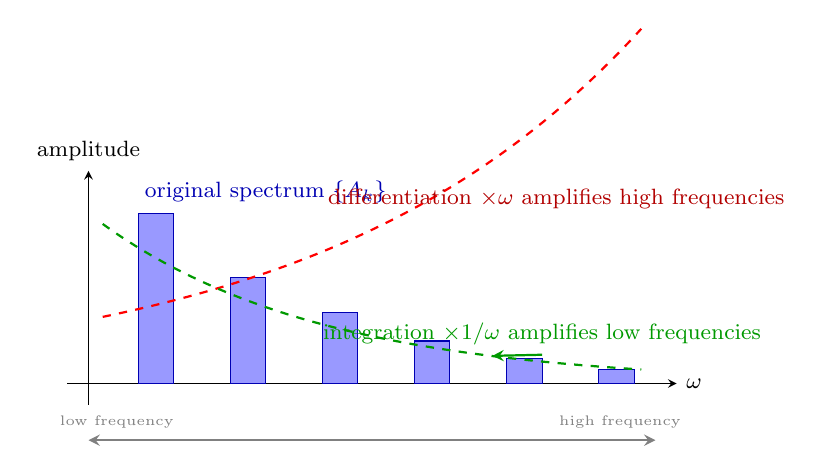
\begin{tikzpicture}[>=stealth, scale=0.9]

    \draw[->] (-0.3,0) -- (8.3,0) node[right, font=\footnotesize] {$\omega$};
    \draw[->] (0,-0.3) -- (0,3.0) node[above, font=\footnotesize] {amplitude};

    \foreach \x/\h in {0.7/2.4, 2.0/1.5, 3.3/1.0, 4.6/0.6, 5.9/0.35, 7.2/0.2} {
        \fill[blue!40] (\x,0) rectangle (\x+0.5,\h);
        \draw[blue!70!black] (\x,0) rectangle (\x+0.5,\h);
    }
    \node[font=\footnotesize, blue!70!black] at (2.5,2.7)
        {original spectrum $\{A_k\}$};

    \draw[thick, red, dashed, domain=0.2:7.8, samples=100]
        plot (\x, {0.9*exp(0.22*\x)});
    \node[font=\footnotesize, red!70!black] at (6.6,2.6)
        {differentiation $\times \omega$ amplifies high frequencies};

    \draw[thick, green!60!black, dashed, domain=0.2:7.8, samples=100]
        plot (\x, {2.4*exp(-0.32*\x)});

    \node[font=\footnotesize, green!60!black] (labInt) at (6.4, 0.7)
        {integration $\times 1/\omega$ amplifies low frequencies};
    \draw[->, thick, green!60!black] (labInt.south)
        -- (5.7, 0.39);

    \draw[<->, thick, gray] (0,-0.8) -- (8.0,-0.8);
    \node[font=\tiny, gray] at (0.4,-0.55) {low frequency};
    \node[font=\tiny, gray] at (7.5,-0.55) {high frequency};
\end{tikzpicture}
\caption{The direction--tendency duality in the frequency domain. Differentiation amounts to multiplication by $\omega$, amplifying high-frequency components; integration amounts to multiplication by $1/\omega$, amplifying low-frequency components. This agrees with the qualitative conclusion of this chapter that `differentiation amplifies high-frequency direction and integration amplifies low-frequency tendency'.}
\label{fig:direction_trend_duality_freq}
\end{figure}

\section{\texorpdfstring{Logarithmic Derivative and the Exponential Map}{Logarithmic Derivative}}

\begin{definition}[Logarithmic derivative]\label{def:log_derivative}
Let $f$ be differentiable at $x$ with $f(x) > 0$. The \textbf{logarithmic derivative} of $f$ is defined as
\[\frac{d}{dx} \ln f(x) = \frac{f'(x)}{f(x)}.\]
\end{definition}

\begin{proposition}[The logarithmic derivative maps scaling to translation]\label{prop:log_derivative_scaling}
\begin{enumerate}[label=(\roman*)]
    \item \textbf{Product conversion}: $(\ln(fg))' = (\ln f)' + (\ln g)'$.
    \item \textbf{Power conversion}: $(\ln f^\alpha)' = \alpha (\ln f)'$.
    \item \textbf{Scaling invariance}: $(\ln(cf))' = (\ln f)'$. Enlarging or shrinking the values of a function does not affect its logarithmic derivative.
\end{enumerate}
The logarithmic derivative is the analytic tool that converts multiplicative scaling ($1$-symmetry) into additive translation ($0$-symmetry).
\end{proposition}

\begin{proof}
(i) By the chain rule and the properties of the logarithmic function:
\[
(\ln(fg))' = \frac{(fg)'}{fg} = \frac{f'g + fg'}{fg} = \frac{f'}{f} + \frac{g'}{g} = (\ln f)' + (\ln g)'.
\]

(ii) By the chain rule:
\[
(\ln f^\alpha)' = \frac{(f^\alpha)'}{f^\alpha} = \frac{\alpha f^{\alpha-1} f'}{f^\alpha} = \alpha \frac{f'}{f} = \alpha(\ln f)'.
\]

(iii) By (i), $(\ln(cf))' = (\ln c)' + (\ln f)' = 0 + (\ln f)' = (\ln f)'$, since $\ln c$ is a constant whose derivative is zero.
\end{proof}

\begin{example}[Exponential growth and the logarithmic derivative]\label{ex:exponential_log_derivative}
The logarithmic derivative of $P(t) = P_0 e^{kt}$ is
\[
(\ln P)' = \frac{P'}{P} = \frac{P_0 k e^{kt}}{P_0 e^{kt}} = k.
\]
Exponential growth is a constant growth rate in the proportional domain, and manifests as uniform translation in the logarithmic domain.
\end{example}

\begin{figure}[htbp]
\centering
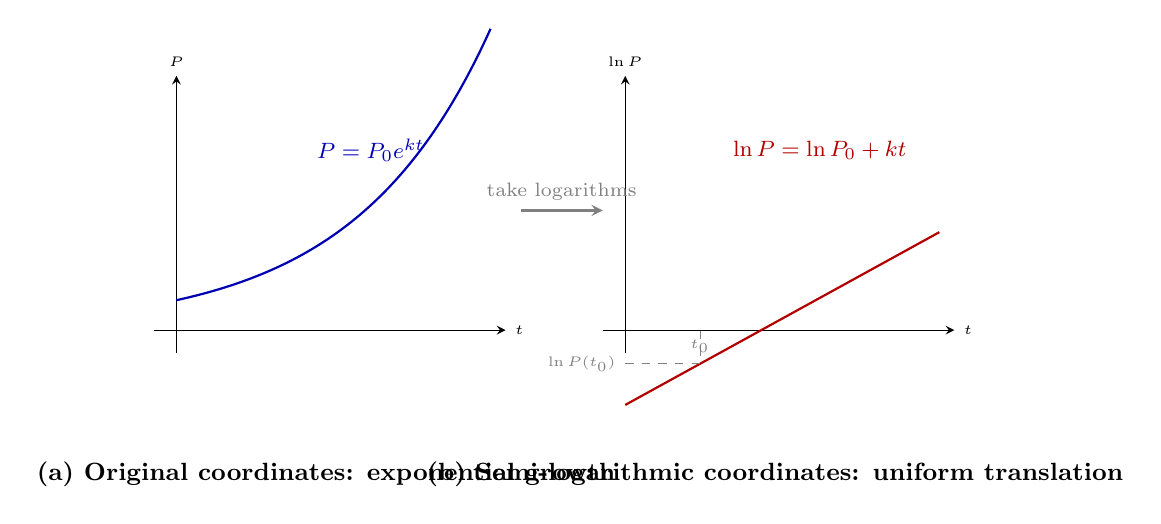
\begin{tikzpicture}[>=stealth, scale=0.95]

    \begin{scope}[shift={(0,0)}]
        \draw[->] (-0.3,0) -- (4.4,0) node[right, font=\tiny] {$t$};
        \draw[->] (0,-0.3) -- (0,3.4) node[above, font=\tiny] {$P$};
        \draw[thick, blue!70!black, domain=0:4.2, samples=100]
            plot (\x, {0.4*exp(0.55*\x)});
        \node[font=\footnotesize, blue!70!black] at (2.6,2.4)
            {$P=P_0 e^{kt}$};
        \node[font=\small\bfseries, below=0.6cm] at (2.0,-1.0)
            {(a) Original coordinates: exponential growth};
    \end{scope}

    \begin{scope}[shift={(6.0,0)}]
        \draw[->] (-0.3,0) -- (4.4,0) node[right, font=\tiny] {$t$};
        \draw[->] (0,-0.3) -- (0,3.4) node[above, font=\tiny] {$\ln P$};
        \draw[thick, red!70!black, domain=0:4.2, samples=100]
            plot (\x, {-1.0 + 0.55*\x});
        \node[font=\footnotesize, red!70!black] at (2.6,2.4)
            {$\ln P=\ln P_0+kt$};
        \draw[dashed, gray] (0,{-1.0+0.55*1.0}) -- (1.0,{-1.0+0.55*1.0})
            -- (1.0,0);
        \node[font=\tiny, gray, left] at (0,{-1.0+0.55*1.0}) {$\ln P(t_0)$};
        \node[font=\tiny, gray, below] at (1.0,0) {$t_0$};
        \node[font=\small\bfseries, below=0.6cm] at (2.0,-1.0)
            {(b) Semi-logarithmic coordinates: uniform translation};
    \end{scope}

    \draw[->, thick, gray] (4.6,1.6) -- (5.7,1.6)
        node[midway, above, font=\scriptsize] {take logarithms};
\end{tikzpicture}
\caption{The logarithmic derivative turns scaling into translation. The left figure shows exponential growth $P=P_0e^{kt}$; after taking logarithms, the right figure becomes the straight line $\ln P=\ln P_0+kt$. This step converts multiplication (proportional scaling) into addition (translation), which is precisely the geometric meaning of the logarithmic derivative $(\ln f)'=f'/f$.}
\label{fig:log_derivative_scaling}
\end{figure}

\section*{Seven-theme comparison table for this chapter}

\begin{center}
\begin{tabular}{>{\centering\arraybackslash}p{2.2cm}>{\centering\arraybackslash}p{10.5cm}}
\toprule
Theme & Corresponding content in this chapter \\
\midrule
Translation & The derivative (directional information) and the limit angle $\theta_f(a)=\arctan f'(a)$ (the section on derivatives, the section on the limit angle) \\
Scaling & The integral (tendency information) and the logarithmic derivative (the conversion between $1$-symmetry and $0$-symmetry, the section on the logarithmic derivative) \\
Rotation & Rotational closure $f^n=\text{id}$ (the section on properties of functions); the behaviour of the limit angle under rotational transformations (the section on the limit angle) \\
Conservation & The fundamental theorem of calculus (the dual conservation of direction and tendency, theorem \ref{thm:ftc}) \\
Symmetry & The parity decomposition theorem (additive reflection symmetry $c=0$, theorem \ref{thm:parity_decomposition}) \\
Closure & Rotational closure $f^n=\text{id}$ corresponds to the finite cyclic group $C_n$ (proposition \ref{prop:rotation_closure_bijective}) \\
Period & The three basic period types (definition \ref{def:periodicity}); the monotone-interval structure of periodic functions (theorem \ref{thm:periodic_monotone_intervals}) \\
\bottomrule
\end{tabular}
\end{center}

\begin{figure}[htbp]
\centering
\adjustbox{max width=\textwidth}{%
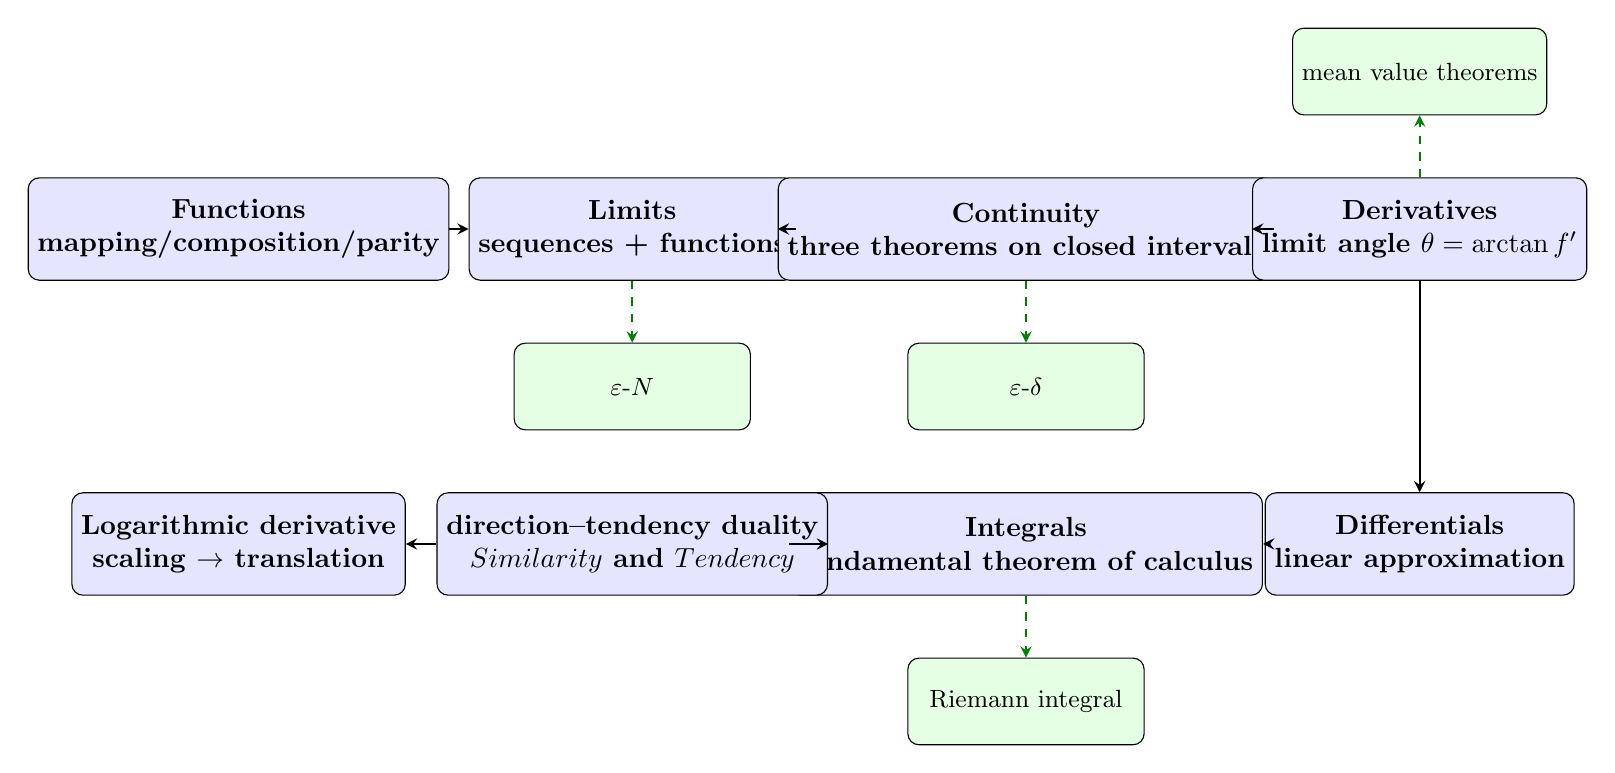
\begin{tikzpicture}[>=stealth,
    main/.style={draw, rounded corners=4pt, fill=blue!10,
        minimum width=3.4cm, minimum height=1.3cm,
        align=center, font=\normalsize\bfseries},
    aux/.style={draw, rounded corners=4pt, fill=green!10,
        minimum width=3.0cm, minimum height=1.1cm,
        align=center, font=\small},
    arrow/.style={-{stealth}, thick},
    auxarrow/.style={-{stealth}, thick, dashed, green!50!black}]

    \node[main] (fun)  at (0,0)    {Functions\\mapping/composition/parity};
    \node[main] (lim)  at (5.0,0)  {Limits\\sequences + functions};
    \node[main] (cont) at (10.0,0) {Continuity\\three theorems on closed intervals};
    \node[main] (der)  at (15.0,0) {Derivatives\\limit angle $\theta=\arctan f'$};

    \node[main] (dif)  at (15.0,-4.0) {Differentials\\linear approximation};
    \node[main] (int)  at (10.0,-4.0) {Integrals\\fundamental theorem of calculus};
    \node[main] (dual) at (5.0,-4.0)  {direction--tendency duality\\$\operatorname{Similarity}$ and $\operatorname{Tendency}$};
    \node[main] (log)  at (0,-4.0)    {Logarithmic derivative\\scaling $\to$ translation};

    \draw[arrow] (fun)  -- (lim);
    \draw[arrow] (lim)  -- (cont);
    \draw[arrow] (cont) -- (der);
    \draw[arrow] (der)  -- (dif);  
    \draw[arrow] (dif)  -- (int);  
    \draw[arrow] (int)  -- (dual);
    \draw[arrow] (dual) -- (log);

    \node[aux] (epsN) at (5.0,-2.0)  {$\varepsilon$-$N$};
    \node[aux] (epsD) at (10.0,-2.0) {$\varepsilon$-$\delta$};
    \node[aux] (mid)  at (15.0,2.0)  {mean value theorems};
    \node[aux] (riem) at (10.0,-6.0) {Riemann integral};

    \draw[auxarrow] (lim)  -- (epsN);
    \draw[auxarrow] (cont) -- (epsD);
    \draw[auxarrow] (der)  -- (mid);
    \draw[auxarrow] (int)  -- (riem);

\end{tikzpicture}}
\caption{Overall map of the logical structure of this chapter (serpentine loop layout). Function theory is the starting point; limits and continuity provide the language of `infinite approximation'; the derivative (direction) and the integral (tendency) are the core analytic tools; the fundamental theorem of calculus places the two in duality; and the logarithmic derivative converts scaling into translation, paving the way for the next chapter, `Differential Equations and Analysis'.}
\label{fig:function_chapter_overview}
\end{figure}

\section*{Exercises}

\begin{enumerate}[leftmargin=3em, label=\textbf{Exercise \arabic*}]
    \item Prove the order-reversal law for the composition of inverse functions (proposition \ref{prop:inverse_composition_order}):
    if $f:X\to Y$ and $g:Y\to Z$ are both bijections, then
    \[
    (g\circ f)^{-1}=f^{-1}\circ g^{-1}.
    \]
    Verify the left inverse and the right inverse separately, and give a concrete example showing that this order is not commutative.

    \item Prove the parity decomposition theorem (theorem \ref{thm:parity_decomposition}):
    any function $f$ defined on a set symmetric about the origin can be decomposed uniquely as
    \[
    f=f_{\text{odd}}+f_{\text{even}},\qquad
    f_{\text{odd}}(x)=\frac{f(x)-f(-x)}{2},\quad
    f_{\text{even}}(x)=\frac{f(x)+f(-x)}{2}.
    \]
    Verify existence and uniqueness separately, and write down the odd part and the even part for $f(x)=e^x$.

    \item Prove that rotational closure implies bijectivity (proposition \ref{prop:rotation_closure_bijective}):
    if $f:X\to X$ satisfies $f^n=\operatorname{id}_X$ ($n\ge1$),
    then $f$ is a bijection and $f^{-1}=f^{n-1}$.
    Further explain the meaning of the statement in note \ref{rem:composition_rotation} that `function composition is itself not a rotation but a translation',
    and explain why $f^n=\operatorname{id}$ corresponds to a finite-order action in a function space.

    \item Prove the theorem on the monotone intervals of a periodic function within its least positive period (theorem \ref{thm:periodic_monotone_intervals}):
    let $f$ be continuous with least positive period $T$; if $f$ is non-constant,
    then in any closed interval of length $T$, $f$ has at least one strictly monotone increasing interval and one strictly monotone decreasing interval.
    Complete the proof using the extreme value theorem and proof by contradiction, and draw a sketch of a periodic function satisfying the conditions.

    \item Prove the boundedness of a convergent sequence (proposition \ref{prop:convergent_bounded}):
    if the sequence $\{a_n\}$ converges, then $\{a_n\}$ is bounded.
    Write out the full details of the $\varepsilon$-$N$ proof, and give an example showing that a bounded sequence need not converge.

    \item Prove that differentiability implies continuity (proposition \ref{prop:diff_implies_cont}),
    and give the counterexample of a continuous but non-differentiable function (note \ref{rem:continuous_not_differentiable}):
    $f(x)=|x|$ is continuous but not differentiable at $x=0$.
    Compute its left and right derivatives and show that the two are unequal.

    \item Prove Fermat's lemma (theorem \ref{thm:fermat}):
    if $f$ is differentiable at $x_0$ and attains a local extremum at $x_0$, then $f'(x_0)=0$.
    Discuss the two cases of a local maximum and a local minimum separately,
    and explain the role of this lemma in the proof of Rolle's theorem (theorem \ref{thm:rolle}).

    \item Prove Rolle's theorem (theorem \ref{thm:rolle}) and Lagrange's mean value theorem (theorem \ref{thm:lagrange}),
    and explain how the latter is deduced from the former by constructing an auxiliary function.
    Further prove the mean value property of periodic functions (corollary \ref{cor:periodic_mean_value}):
    if $f$ is differentiable with period $T$, then within one period there exists $\xi$ such that $f'(\xi)=0$.

    \item Let $f(x)=x^3-3x+1$. Compute:
    \begin{enumerate}[label=(\roman*)]
        \item the derivative $f'(1)$ of $f$ at $x=1$;
        \item the limit angle $\theta_f(1)=\arctan f'(1)$ at that point;
        \item the limit angle $\theta_g(0)$ of $g(x)=\sin x$ at $x=0$;
        \item the differential-difference similarities of the two at the point $(1,0)$,
              $\operatorname{Similarity}_{\text{value}}(f,g;1,0)$ and
              $\operatorname{Similarity}_{\text{dir}}(f,g;1,0)$ (definition \ref{def:diff_similarity}).
    \end{enumerate}

    \item Prove the second part of the fundamental theorem of calculus (theorem \ref{thm:ftc}):
    if $F$ is any antiderivative of $f$, then
    \[
    \int_a^b f(x)\,dx=F(b)-F(a).
    \]
    Complete the proof using the integral with variable upper limit $\Phi(x)=\int_a^x f(t)\,dt$ and Lagrange's mean value theorem,
    and explain the mutual invertibility of differentiation and integration in corollary \ref{cor:diff_int_inverse}.

    \item Prove that the logarithmic derivative converts scaling into translation (proposition \ref{prop:log_derivative_scaling}):
    \begin{enumerate}[label=(\roman*)]
        \item $(\ln(fg))'=(\ln f)'+(\ln g)'$;
        \item $(\ln f^\alpha)'=\alpha(\ln f)'$;
        \item $(\ln(cf))'=(\ln f)'$.
    \end{enumerate}
    Taking $P(t)=P_0e^{kt}$ as an example (example \ref{ex:exponential_log_derivative}),
    verify that its logarithmic derivative is the constant $k$, and explain how this expresses a `constant growth rate in the proportional domain'.

    \item Prove the theorem on the equality of mixed partial derivatives (theorem \ref{thm:clairaut}):
    if $f_{xy}$ and $f_{yx}$ are continuous on a neighbourhood of $(x_0,y_0)$,
    then $f_{xy}(x_0,y_0)=f_{yx}(x_0,y_0)$.
    Write out the derivation of the second-order difference $\Delta(h,k)$, and explain that the continuity hypothesis cannot be omitted
    (see the counterexample \ref{rem:partial_not_differentiable}).

    \item Synthesis question: explain how the limit angle
    \[
    \theta_f(a)=\arctan f'(a)
    \]
    connects the geometric argument at the vector level with the calculus direction at the function level.
    Using definition \ref{def:limit_angle}, proposition \ref{prop:limit_angle_properties}
    and proposition \ref{prop:limit_angle_transformations},
    discuss the behaviour of the limit angle under the three basic transformations of translation, scaling and rotation,
    and point out its significance in the analysis of periodic functions.
\end{enumerate}

